\chapter{Probabilistic models of dialogue}
\label{chap:probmodelling}

The previous chapter provided an overview of the most influential approaches to dialogue management, and outlined in particular the benefits of statistical techniques to account for the uncertainty and unpredictability inherent to spoken dialogue. The present chapter exposes the theoretical and methodological foundations of these statistical approaches as well as their application to the dialogue management task. 

The first section of this chapter concentrates on the use of graphical models to design structured representations of probability and utility distributions. Graphical models provide mathematically principled methods for representing, estimating and reasoning over complex probabilistic domains. The section starts with the most well-known type of directed graphical model, namely Bayesian networks.  We then show how to extend Bayesian networks to capture temporal sequence and express decision-theoretic problems through actions and utilities. We also review the most important inference and learning algorithms developed for these graphical models.

Based on these graphical models, the second section presents the fundamental principles of reinforcement learning, which is the learning framework employed by most statistical approaches to dialogue management. The section starts with a definition of Markov Decision Processes and explains how policies can be automatically optimised for such processes.  The discussion is then extended to partially observable environments in which the current state is hidden and must be indirectly inferred from observations.   

Once the mathematical foundations of graphical models and reinforcement learning are in place, the third and last section of this chapter describe how these concepts and techniques can be practically applied to model dialogue management tasks.  The section provides a survey of the multiple approaches that have been developed in the last two decades to automatically optimise dialogue policies based on various flavours of supervised and reinforcement learning.  

\section{Graphical models}
\label{sec:pgm}

We describe in this section the core properties of (directed) graphical models,\footnote{There also exists a variety of undirected graphical models, amongst which Markov networks, as well as partially directed models (e.g. Conditional Random Fields), but they will not be discussed nor employed in this thesis.} their formal representation, and their use in learning and inference tasks. 
 
 \subsection{Representations}
 \label{sec:gm-representation}
\subsubsection*{Bayesian networks}

Let $\mathbf{X} = X_1 ... X_n$ denote a set of random variables, where each variable $X_i$ is associated with a range of mutually exclusive values.  This range can be either discrete or continuous.  For dialogue models, the range of a variable $X_i$ is typically discrete and can be explicitly enumerated. The enumeration of values for the variable $X_i$ can be written $Val(X_i) = \{x_i^1, ..., x_i^m\}$.  

In the general case, the variables $\mathbf{X}$ can be interrelated by complex probabilistic dependencies.  These dependencies can be expressed through the joint probability distribution $P(X_1 ... X_n)$.  The size of this joint distribution is however exponential in the number $n$ of variables, and is therefore difficult to manipulate (let alone estimate and reason over) directly. 

% In dialogue models, this range is often discrete and can be explicitly enumerated: $Val(X_i) = \{x_i^1, ..., x_i^m\}$.  

It is fortunately possible to exploit conditional independence properties to reduce the complexity of the joint probability distribution.  For three disjoint sets of random variables $\mathbf{X}$, $\mathbf{Y}$ and $\mathbf{Z}$, we say that $\mathbf{X}$ and $\mathbf{Y}$ are conditionally independent given $\mathbf{Z}$ iff $P(\mathbf{X},\mathbf{Y} \, | \, \mathbf{Z}) = P(\mathbf{X} \, | \, \mathbf{Z}) P(\mathbf{Y} \, | \, \mathbf{Z})$ for all possible combination of values for  $\mathbf{X}$, $\mathbf{Y}$ and  $\mathbf{Z}$. This conditional independence is denoted $(\mathbf{X} \ \bot \  \mathbf{Y} \, | \,  \mathbf{Z})$. 

Conditional independence allows a joint probability distribution to be decomposed into smaller distributions that are much easier to work with.  For a variable $X_i$ in $ X_1...X_n$, we can define the set $parents(X_i)$ as the minimal set of predecessors of $X_i$ such that the other predecessors of $X_i$ are conditionally independent of $X_i$ given $parents(X_i)$.  The set of parents can be empty if the variable $X_i$ is independent of all other variables. This definition enables us to decompose the joint distribution based on the chain rule:
\begin{align}
P(X_1,...X_n) & = \ \prod_{i=1}^n P(X_i  \, | \,  X_1, ... X_{i-1}) \\
&= \ \prod_{i=1}^n P(X_i  \, | \,  parents(X_i)) 
\end{align}

This decomposition can be graphically represented in a \textit{Bayesian network}.  A Bayesian network is a directed acyclic graph (DAG) where each random variable is represented by a distinct node.  These nodes are connected via directed edges that reflect conditional dependencies. In other words, an edge $X_m \rightarrow X_n$ indicates that $X_m \in parents(X_n)$. Each variable $X_i$ in the Bayesian network must be associated with a specific conditional probability distribution $P(X_i  \, | \,  parents(X_i))$.   Together with the directed graph, the conditional probability distributions (abbreviated as CPDs) fully determine the joint probability distribution of the Bayesian network.   

Given such definitions, the Bayesian network can be directly used for inference by querying the distribution of a subset of variables, often given some additional evidence. Two operations are especially useful when manipulating probability distributions: 
\begin{itemize}
\item Marginalisation (also called ``summing out''), which derives the probability of the variable $X$ given its conditional distribution $P(X \, | \, Y)$ and the distribution $P(Y)$: 
\begin{align}
P(X) & = \ \sum_{y \in Val(Y)} P(X,Y) = \ \sum_{y \in Val(Y)} P(X \, | \, Y) P(Y)
\end{align}
\item Bayes' rule, which reverses the order of a conditional distribution between two variables $X$ and $Y$ (possibly with some background evidence $\mathbf{e}$): 
\begin{equation}
P(X \, | \, Y, \mathbf{e}) = \frac{P(Y \, | \, X, \mathbf{e}) P(X \, | \, \mathbf{e})} {P(Y \, | \, \mathbf{e})} \label{eq:genbayes}
\end{equation}
\end{itemize}

As an illustration, Figure \ref{fig:plainbn} provides an example of Bayesian network that models the probability of occurrence of a fire at a given time.  The probability of this event is dependent on the current weather.  In addition, two (imperfect) monitoring systems are used to detect possible fires; one on the ground, and one via satellite.  

\begin{figure}[h]
\centering
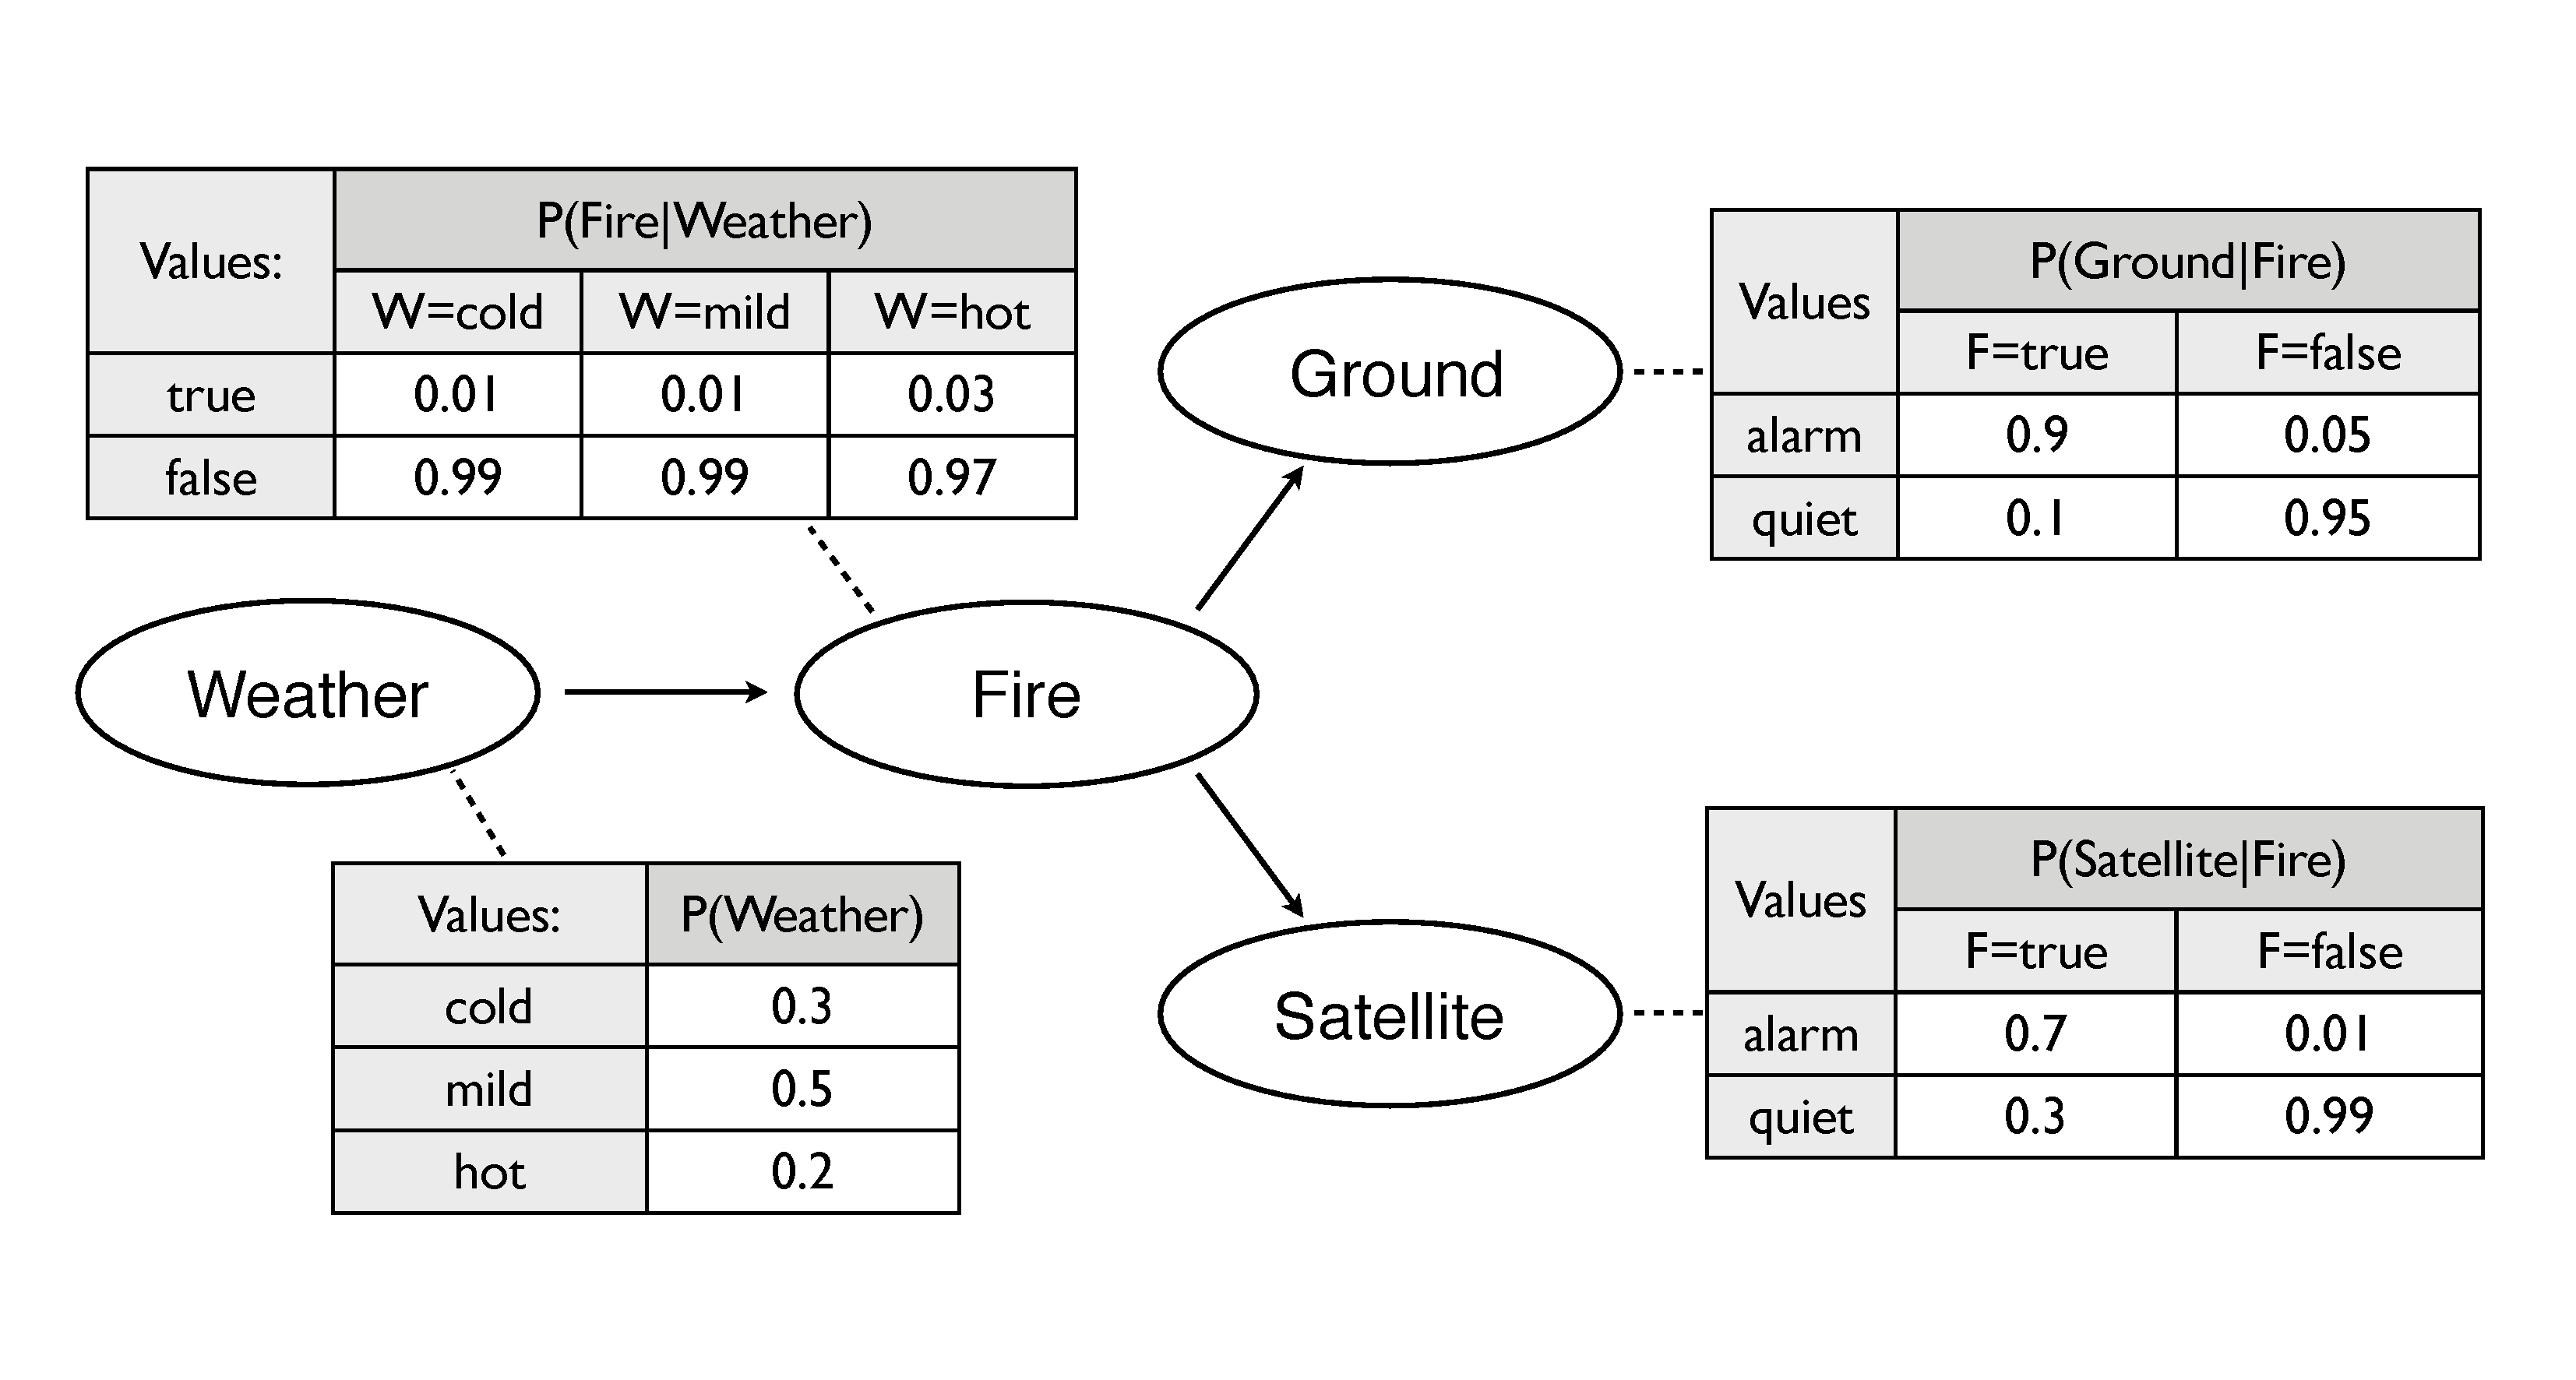
\includegraphics[scale=0.25]{imgs/plainbn.pdf}
\caption{Example of Bayesian network with four random variables.}
\label{fig:plainbn}
\end{figure}

% \begin{example}
%Based on the network in Figure \ref{fig:plainbn}, we can calculate the probability of a fire given that a fire has been reported on the ground but not via satellite, and that the weather is mild.\footnote{Variable names and values are abbreviated to their first letter for better readability.} Applying Bayes' rule shown in Equation \ref{eq:genbayes}, we can derive: 
%\begin{align}
%P(F \, | \, W\!=\!m, G\!=\!y, S\!=\!n) & = \frac{P(G\!=\!y, S\!=\!n \, | \, F,W\!=\!m) \, P(F \, | \, W\!=\!m)} {P(G\!=\!y, S\!=\!n \, | \, W\!=\!m)} \label{eq:example11} \\
%\intertext{Since $(T \ \bot \ A \, | \,  F)$, we can further simplify: }
%& = \frac{P(G\!=\!y \, | \, F) \, P(S\!=\!n \, | \, F) \, P(F \, | \, W\!=\!m)} {P(G\!=\!y, S\!=\!n \, | \, W\!=\!m)} \\
%\intertext{As the only function of the denominator is to normalise the final probabilities, it can be replaced by a normalisation constant $\alpha$:}
%& = \alpha \, P(G\!=\!y \, | \, F) \, P(S\!=\!n \, | \, F) \, P(F \, | \, W\!=\!m)  \label{eq:example12}
%\end{align}

%Given Equation \ref{eq:example12}, the probability of a fire becomes $\alpha \times 0.9 \times 0.3 \times 0.01$, while the probability of the absence of fire is $\alpha \times 0.05 \times 0.99 \times 0.99$.  After normalisation, the final probability of a fire is then estimated to be $\approx 0.052$.  \qed \\[-4mm]
%\end{example}

There is one distinct distribution for every combination of values in $parents(X_i)$. The probabilistic model defined in the figure includes therefore a total of eight distributions.  The distributions in Figure \ref{fig:plainbn} are \textit{categorical} distributions.\footnote{Categorical distributions are often conflated with \textit{multinomial} distributions, which specify the number of times an event will occur in a repeated independent trial with $k$ exclusive categories, with each category having a fixed probability.  A categorical distribution is equivalent to a multinomial distribution for a single observation.} Categorical distributions can be encoded with look-up tables that map every possible value in $Val(X_i)$ to a particular probability.  Many of the probability distributions used throughout this thesis will take the form of categorical distributions. Other representations for discrete CPDs are however conceivable, as will be shown later in this thesis.

A Bayesian network can also contain continuous probability distributions.  These distributions are usually encoded with \textit{density functions} represented in a parametric form.  A well-known example of parametric distribution is the normal distribution $\mathcal{N}(\mu,\sigma^2)$, which is defined by its two parameters $\mu$ (the mean) and $\sigma^2$ (the variance). Continuous distributions can alternatively expressed with non-parametric methods based on e.g. kernel estimators.  The reader is invited to consult  \cite{Bishop:2006} and \cite{Koller+Friedman:09} for more detail on these distributions. 

Appendix \ref{chap:probdistributions} enumerates the most important discrete and continuous probability distributions employed in this thesis.  %Finally, hybrid probabilistic models involving both discrete and continuous variables can be defined. 

\subsubsection*{Reasoning over time}

In order to apply Bayesian networks to tasks such as dialogue management, two additional elements are necessary. The first extension is to allow variables to evolve as a function of time.  Such temporal dependencies are indeed necessary to account for the dynamic nature of dialogue (the dialogue state is not a static entity but is expected to change over time). Two assumptions are usually made to structure such temporal dependencies: \begin{enumerate}
\item The first assumption, called the Markov assumption, is that the variable values at time $t$ only depend on the previous time slice $t\!-\!1$.  Formally, let $\mathbf{X}$ be an arbitrary collection of variables. We denote by $\mathbf{X}_t$ the random variables that express their values at time $t$.  The Markov assumption states that $(\mathbf{X}_t \; \bot \; \mathbf{X}_{0:(t-2)}  \, | \,  \mathbf{X}_{t\!-\!1})$.  

\item The second assumption is that the process is stationary\footnote{A \textit{stationary} process must be distinguished from a \textit{static} process: a static process is a stochastic process that remains constant for all time steps. In contrast, a stationary process can change over time, but the transition model that describes the dynamics of this process remains constant.} -- that is, that the probability $P(\mathbf{X}_t  \, | \,  \mathbf{X}_{t\!-\!1})$ is the same for all values of $t$.
\end{enumerate}

Given these two assumptions, we can define a stochastic process with a probability distribution $P(\mathbf{X}_t  \, | \,  \mathbf{X}_{t\!-\!1})$ that specifies the distribution of the variables $\mathbf{X}$ at time $t$ given their values at time $t\!-\!1$. Such model is called a \textit{dynamic Bayesian network} (DBN). The distribution $P(\mathbf{X}_t  \, | \,  \mathbf{X}_{t\!-\!1})$ can be internally factored and include dependencies both between the time slices $t\!-\!1$ and $t$ and within the slice $t$.  Figure \ref{fig:dbn} shows a concrete example of dynamic Bayesian network. The DBN provides a factored representation of the distribution  $P(R_t, F_t, G_t \, | \, R_{t\!-\!1}, F_{t\!-\!1})$.  

Given the specification of the distribution $P(\mathbf{X}_t  \, | \,  \mathbf{X}_{t\!-\!1})$ and an initial distribution $P(\mathbf{X}_0)$, a dynamic Bayesian network can be ``unrolled'' onto multiple time slices.  This unrolled model corresponds to a classical Bayesian network.  

\begin{figure}[h]
\centering
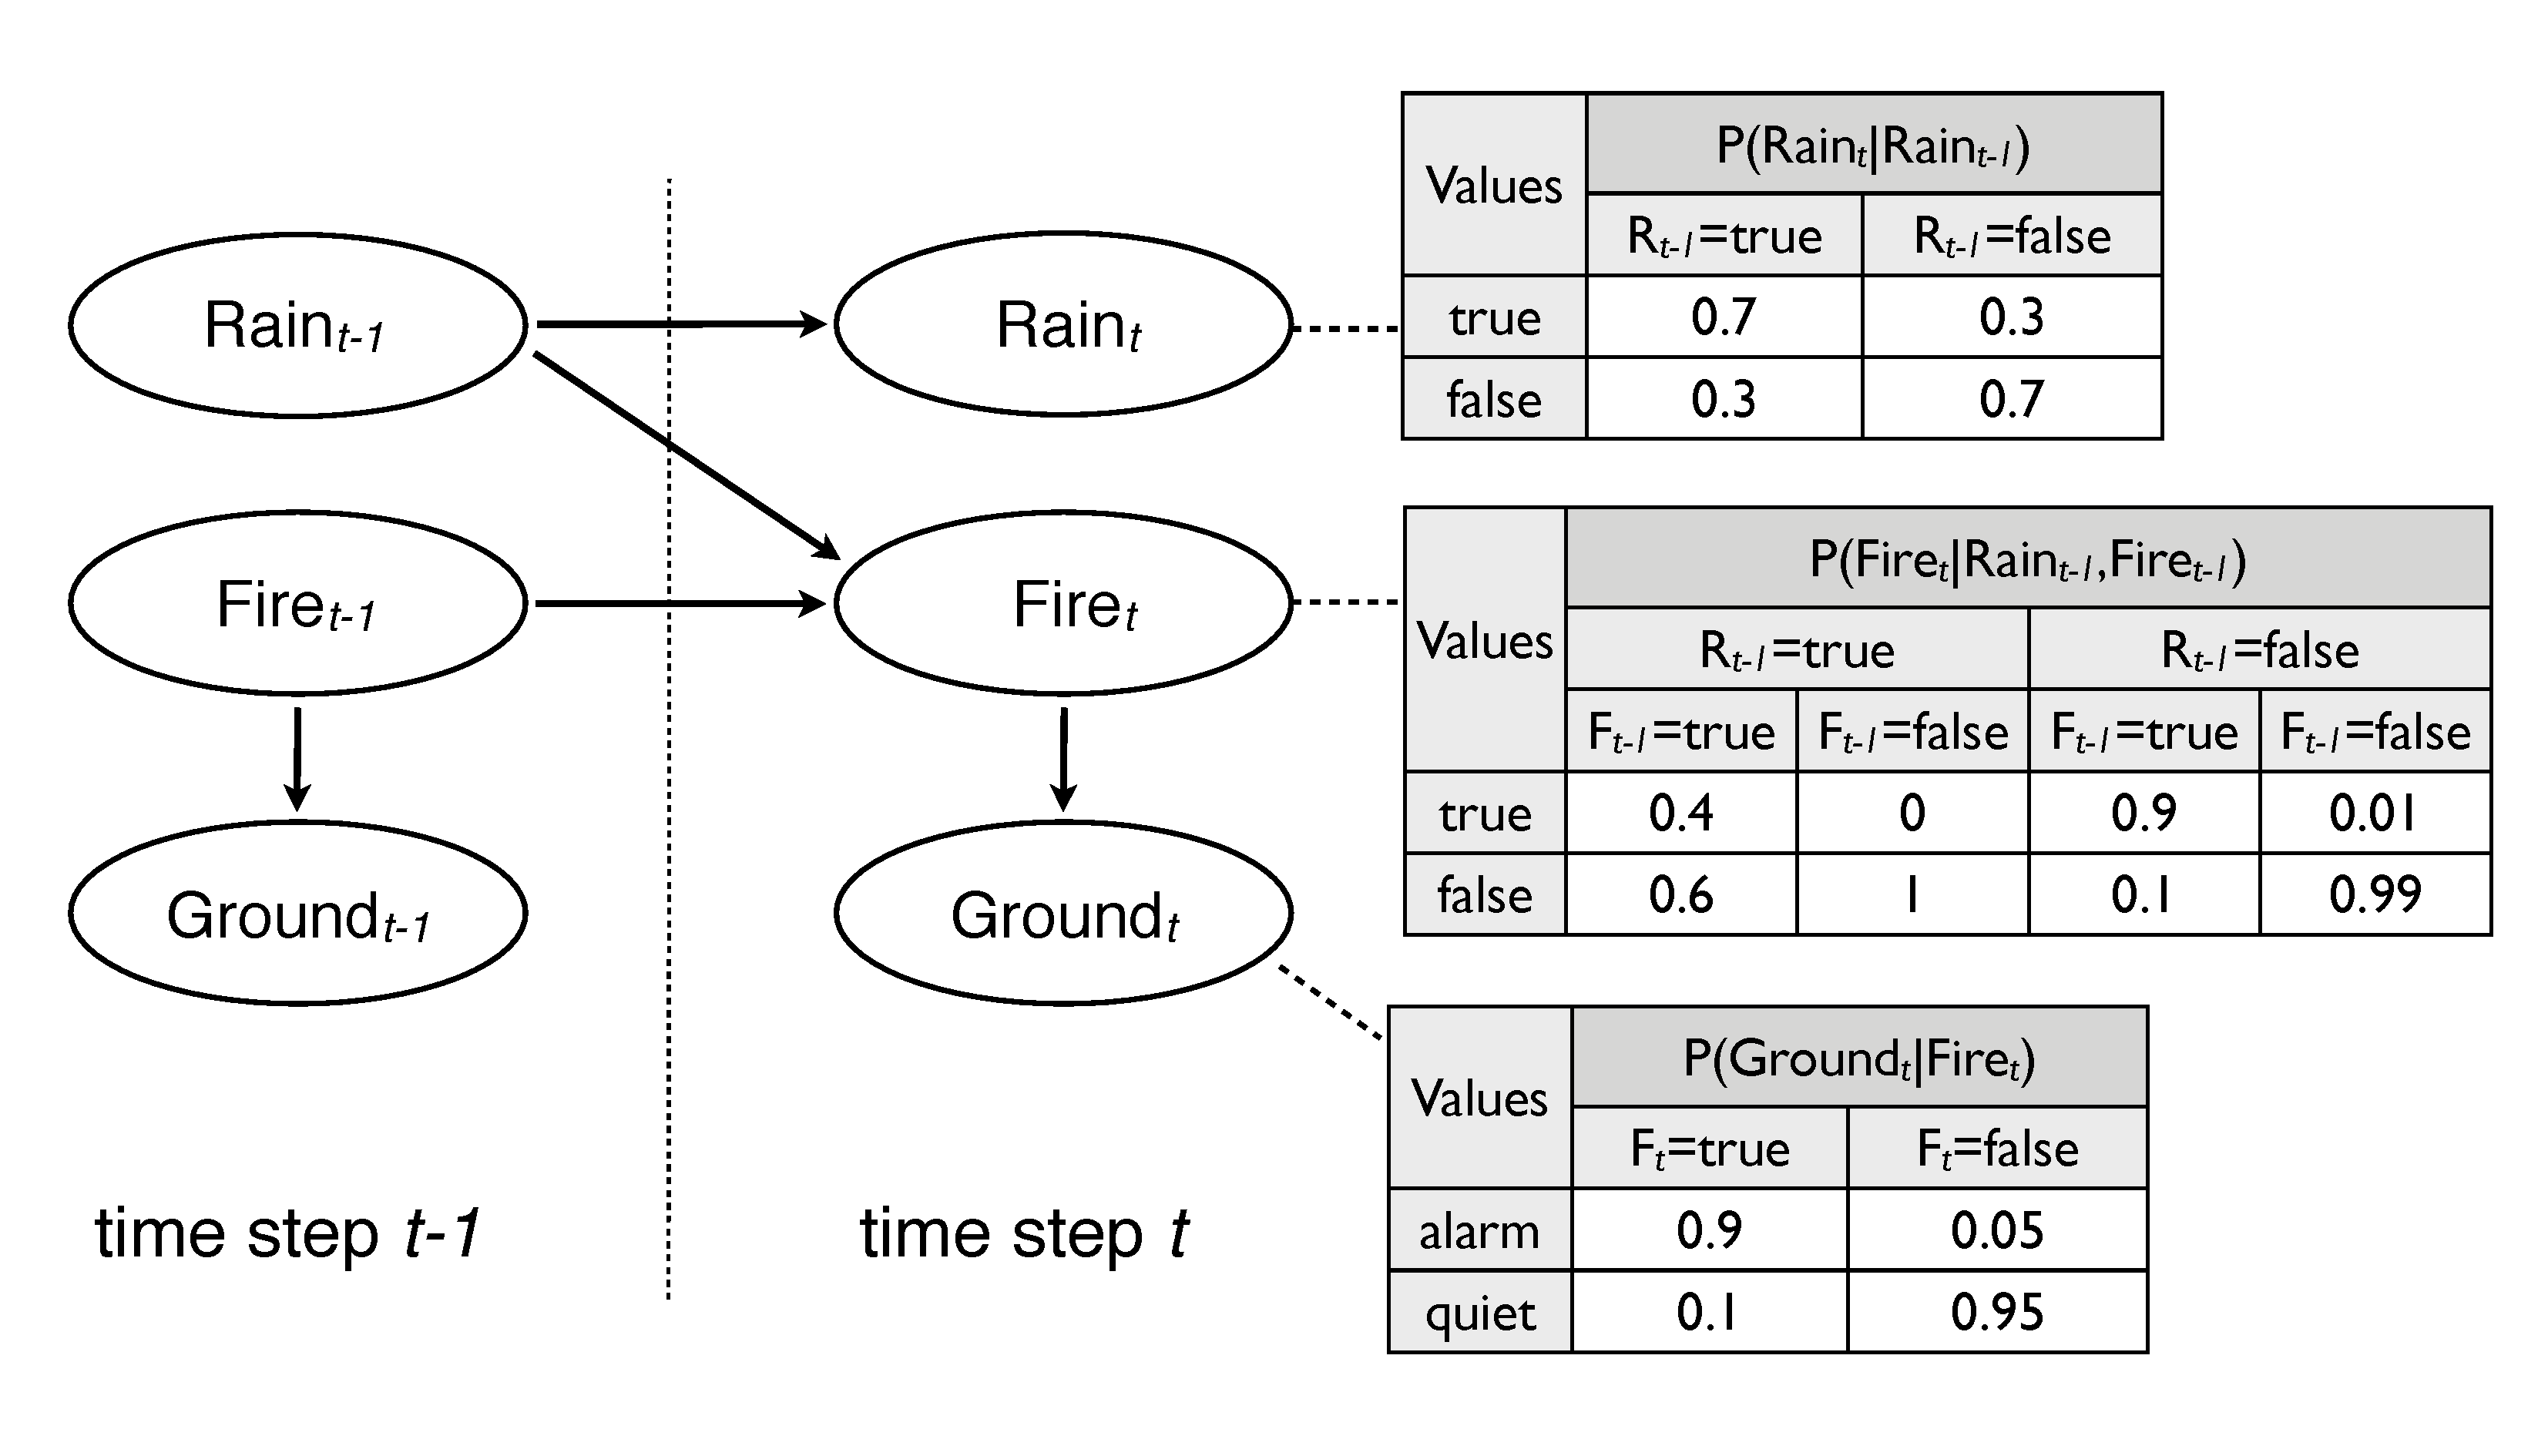
\includegraphics[scale=0.25]{imgs/dbn.pdf}
\caption{Example of dynamic Bayesian network. }
\label{fig:dbn}
\end{figure}

% \begin{example}
%We can calculate the probability of a fire at time $t$, given that we know that the probability of a fire at time $(t\!-\!1=$ is $P(F_{t\!-\!1})\!=\!0.05$ and no rain was recorded at that time.  Using marginalisation, we can derive:
%\begin{align}
%P(F_{t}) & = \ \sum_{w \in Val(F_{t\!-\!1})} \ \  \sum_{r \in Val(R_{t\!-\!1})}  P(F_{t}, F_{t\!-\!1}\!=\!w, R_{t\!-\!1}\!=\!r) \\
%& = \  \sum_{w \in Val(F_{t\!-\!1})} P(F_{t} \, | \, F_{t\!-\!1}\!=\!w, R_{t\!-\!1}\!=\!n) P(F_{t\!-\!1}\!=\!w) \label{eq:dbnexample}
%\end{align}

%Summing up the probabilities for the two possible values of $F_{t\!-\!1}$, Equation \ref{eq:dbnexample} returns the result $P(F_{t} = \mathit{true}) = 0.9 \times 0.05 + 0.01 \times 0.95  \approx 0.055$.  \qed \\[-4mm]
%\end{example}

\subsubsection*{Decision problems}

Dynamic Bayesian networks are well-suited to represent temporal processes.  However, in sequential decision tasks such as dialogue management, tracking the current state is only the first step of the reasoning process. The agent must also be able to calculate the relative utilities of the various actions that can be executed at that  state. The second extension of Bayesian networks thus pertains to the inclusion of actions and utilities in addition to state variables.  

\textit{Decision networks}\footnote{Decision networks are also called \textit{influence diagrams}.} are Bayesian networks augmented with a representation of action variables and their corresponding utilities. Decision networks may include three classes of nodes:
\begin{enumerate}
\item \textit{Chance nodes} correspond to the classical random variables described so far.  Chance nodes are associated with conditional probability distributions that define the relative probabilities of the node values given the values in the parent nodes.
\item \textit{Decision nodes} (sometimes also called action nodes) correspond to variables that are under the control of the system.  The values of these nodes reflect an active choice made by the system to execute particular actions.
\item \textit{Utility nodes} express the utilities (from the system's point of view) associated with particular situations expressed in the node parents.  Typically, these parents combine both chance and decision variables.   Utility nodes are coupled with utility distributions that associate each combination of values in the node parents with a specific (negative or positive) utility. 
\end{enumerate}

Decision networks combined with temporal dependencies are called \textit{dynamic decision networks}.  Figure \ref{fig:ddn} illustrates a dynamic decision network with a decision variable containing two alternative actions assigned to distinct utility values depending on the occurrence of fire. 

%The utility variable $U$ encodes the utility function associated with these two actions depending on the current state of the fire -- in this case, a large positive value ($+5$) if the water is dropped when a fire occurs, a large negative value ($-5$) if no water is dropped when a fire occurs, and a small negative value ($-1$) if the water is dropped in the absence of a fire.  It is also worth noting that $\mathit{Fire}_t$ depends on both the $Fire_{t\!-\!1}$ and the action variable $Tanker_{t-1}$.  The system is therefore able to actively influence the evolution of the state based on its own actions. 
 
\begin{figure}[h]
\centering
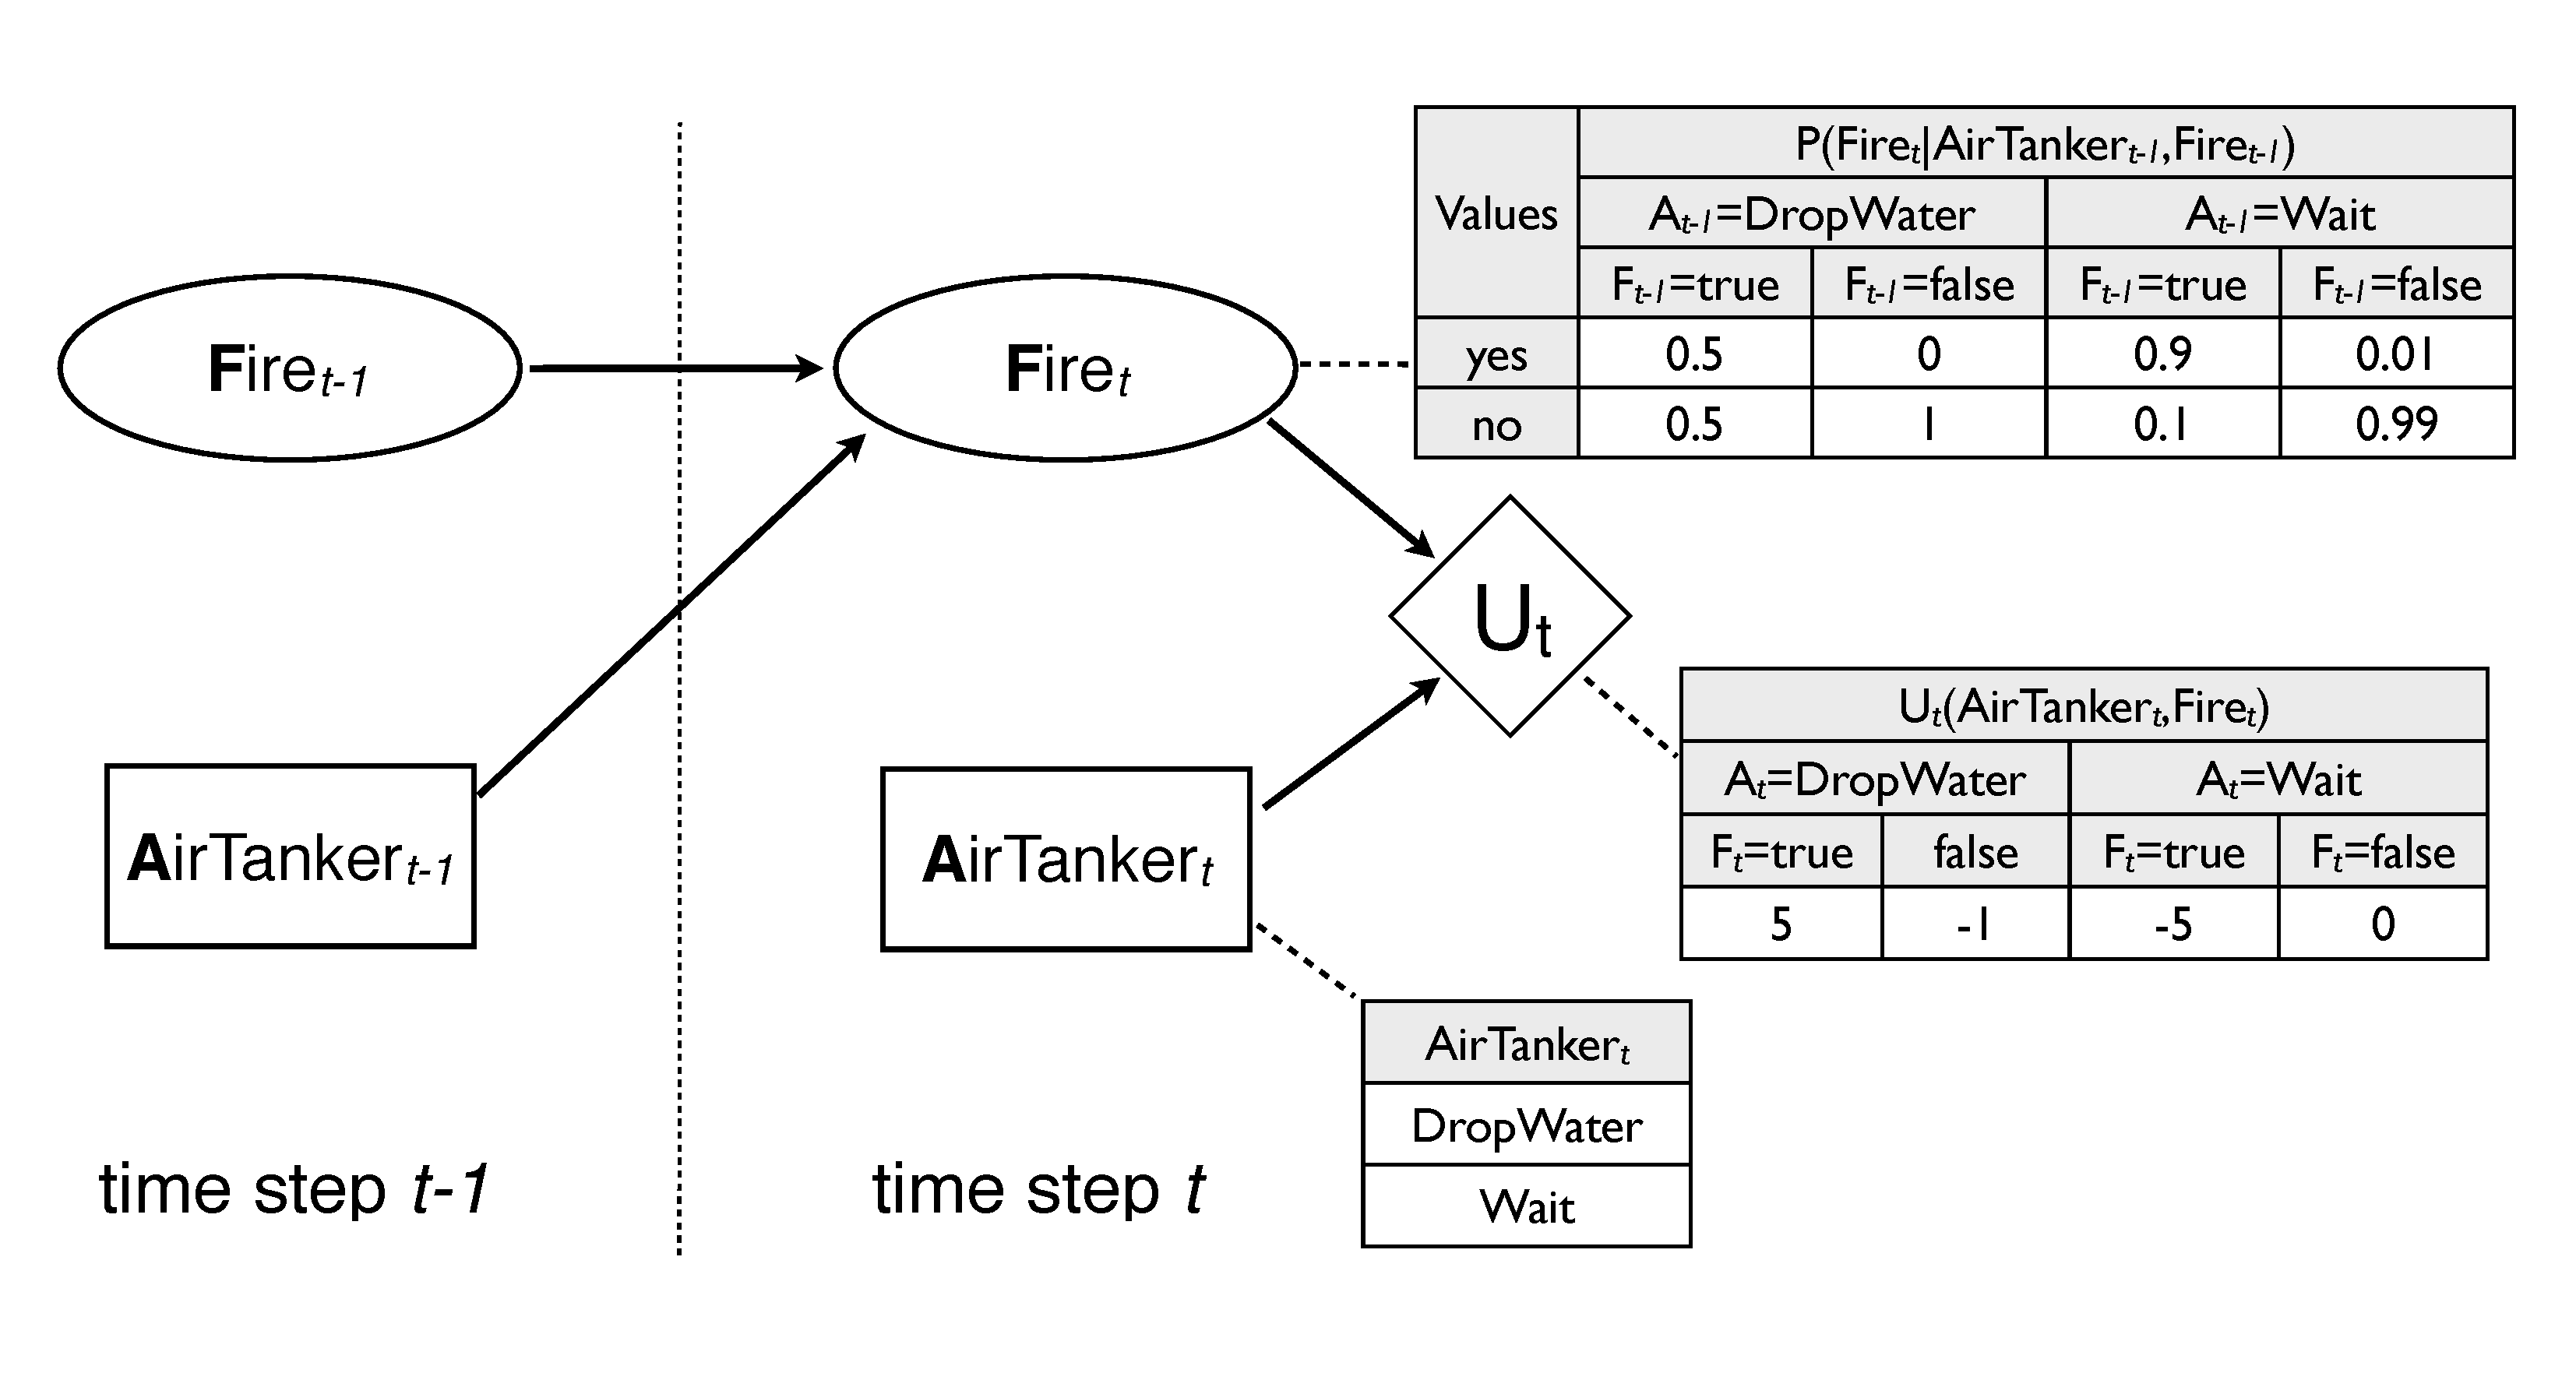
\includegraphics[scale=0.25]{imgs/ddn.pdf}
\caption{Example of dynamic decision network. By convention, chance nodes are represented with circles, decision nodes with squares, and utility nodes with diamonds. }
\label{fig:ddn}
\end{figure}

%\begin{example}
%\label{ex:example3}
%Assuming the probability of a fire at time $t$ is $P(\mathit{Fire}_t) = 0.05$, we can calculate the utility of the two actions $\mathit{DropWater}$ and $\mathit{Wait}$ based on the network in Figure \ref{fig:ddn}:
%\begin{align}
%U_t(A_t) & = \ \sum_{w \in Val(F_t)} U_t(A_t, F_t = w) 
%\end{align}
%For $A_t\!=\!DropWater$, the utility is therefore $0.05 \times 5 - 0.95 = -0.7$, while the utility of $A_t\!=\!Wait$ is equal to $0.05 \times (-5) = -0.25$.  A rational agent will therefore favour the action $A_t = Wait$ in this situation.  \qed \\[-4mm]
%\end{example}

\subsection{Inference} 
\label{sec:inference}
\subsubsection*{Generalities}

The main purpose of probabilistic graphical models is to evaluate \textit{queries} -- that is, calculate a posterior distribution over a subset of variables, usually given some evidence. Assuming a graphical model defining the joint probability distribution of a set of variables $\mathbf{X}$, a probability query is a posterior distribution of the form $P(\mathbf{Q}  \, | \,  \mathbf{E}\!=\!\mathbf{e})$, where $\mathbf{Q} \subset \mathbf{X}$ denotes the query variables, $\mathbf{E} \subset \mathbf{X}$ the evidence variables, and $\mathbf{e}$ a possible assignment of values for the evidence variables.  If the set of evidence variables is empty, the query is reduced to the calculation of a marginal distribution.  Graphical models augmented with decision and utility variables can also be used to answer utility queries of the form $U(\mathbf{Q}   \, | \,  \mathbf{E}\!=\!\mathbf{e})$.  In this case, the query variables often correspond to decision nodes whose utility is to be estimated.

A wide range of inference algorithms have been developed to efficiently evaluate these probability and utility queries. These algorithms can be either exact or approximate.  

Exact algorithms calculate the precise posterior distribution corresponding to the query through a sequence of manipulation operations on the CPDs contained in the graphical model.  One popular algorithm for exact inference is variable elimination \citep{ZhangP96}.  Variable elimination relies on dynamic programming techniques to evaluate a query through a a sequence of matrix operations (summation and pointwise product). These operations are defined on so-called ``factors'' that represent CPDs in a matrix format. Variable elimination can be generalised to handle utility queries using joint factors \citep{Koller+Friedman:09}.   Other algorithms such as message passing on clique trees can also be used \citep{jensen1990}. 

Exact inference remains unfortunately difficult to scale to large, densely interconnected graphical models, and  approximate techniques are often unavoidable in many practical domains.  Algorithms for approximate inference in graphical models include approaches such as loopy belief propagation \citep{Murphy:1999}, variational methods \citep{Jordan:1999},  and a wide array of sampling techniques \citep{mackay1998introduction}, sometimes also called Monte Carlo methods. Popular sampling techniques include various flavours of importance sampling \citep{FungC89,cheng2000ais} and Markov Chain Monte Carlo (MCMC) approaches such as Gibbs sampling \citep{pearl1987evidential,gamerman2006markov}. % In contrast to other approximation methods, sampling can be straightforwardly applied to arbitrary probabilistic models, and notably hybrid models that combine continuous and discrete variables.  Ath are also guaranteed to converge to the correct results at the large sample limit.  Their practical performance can however be difficult to predict for modest sample sizes. 

Probabilistic inference is a difficult computational task.  In fact, inference on unconstrained Bayesian Networks is known to be {\#}P-hard, which is a complexity class that is strictly harder than NP-complete problems.  This holds both for exact inference \citep{Cooper90}, and -- perhaps more surprisingly -- also for approximate inference \citep{Dagum1993}.  


The \opendial toolkit we have developed for this thesis includes two inference algorithms: generalised variable elimination \citep[][p. 1103]{Koller+Friedman:09} and a specific type of importance sampling algorithm called likelihood weighting, which we outline below. These algorithms are used in the processing workflow of the dialogue manager to (1) update the dialogue state upon the reception of new observations and (2) select system actions on the basis of this updated dialogue state. The details of this workflow will be provided in Section \ref{sec:processing-workflow}.  

\subsubsection*{Likelihood weighting} 

To make our discussion of inference algorithms for graphical models more concrete, we describe below a simple but efficient sampling method called \textit{likelihood weighting} \citep{FungC89}, which we have used in most of the experiments conducted in this thesis.  

The key principle behind all types of sampling algorithms is to estimate the posterior distribution expressed in the query by collecting a large quantity of samples (i.e. assignments of values to the random variables) drawn from the graphical model.  Likelihood weighting proceeds by sampling the random variables in the graphical model one by one, in topological order (i.e. from parents to children).\footnote{A partial order on the nodes in the graph can always be found since the network is a directed acyclic graph.} For instance, sampling the network in Figure \ref{fig:plainbn} will start with the variable $\mathit{Weather}$, then $\mathit{Fire}$ (based on the value drawn for the parent $\mathit{Weather}$), and finally $\mathit{Ground}$ and $\mathit{Satellite}$ (based on the value drawn for $\mathit{Fire}$).  In order to account for the evidence $\mathbf{e}$, every sample is associated with a specific \textit{weight} that expresses the likelihood of the evidence given the assignment for all the other variables.  For graphical models that include utility variables, samples also record the total utility accumulated for the sampled values. The pseudocode in Algorithm \ref{algo:getsample} outlines the sampling procedure.  
% (modified from \cite{aima2010,Koller+Friedman:09})

\begin{algorithm}[h!]
\caption{: \textsc{Get-Sample} $(\mathcal{B}, \mathbf{e})$}
\begin{algorithmic}[1] \vspace{2mm} 
\REQUIRE Bayesian/decision network $\mathcal{B}$ over $\mathbf{X}$ with topological ordering $X_1,...X_n$
\REQUIRE Evidence $\mathbf{E} =\mathbf{e}$
\ENSURE Full sample drawn from $\mathcal{B}$ together with a weight and utility \\[2mm]
\STATE Initialise sample $\mathbf{x} \leftarrow \langle \mathbf{e} \rangle$
\STATE Initialise weight $w \leftarrow 1$ and utility $u \leftarrow 0$
\FORALL {$X_i \in X_1,...X_n$} 
\IF {$X_i$ is a chance or decision variable and $X_i \notin \mathbf{E}$}
\STATE $x_i \leftarrow$ sample value drawn from $P(X_i  \, | \,  \mathbf{x})$
\STATE $\mathbf{x} \leftarrow \mathbf{x} \cup \langle x_i \rangle$
\ELSIF {$X_i$ is a chance variable and $X_i \in \mathbf{E}$}
\STATE $w \leftarrow w \times P\left(X_i = \mathbf{e}(X_i)  \, | \,  \mathbf{x}\right)$
\ELSIF {$X_i$ is a utility variable}
\STATE $u \leftarrow u + U_i(\mathbf{x})$
\ENDIF
\ENDFOR
\RETURN $\mathbf{x}, w, u$
\end{algorithmic}
\label{algo:getsample}
\end{algorithm}

The notation $\mathbf{e}(X_i)$ refers to the value specified for the variable $X_i$ in the assignment $\mathbf{e}$. 

A large number of samples can be accumulated in this manner. Once enough samples are collected (or the inference engine has run out of time) the resulting posterior distribution for the query variables $\mathbf{Q}$ is derived by normalising the weighted counts associated with each value of the query variables, as shown in Algorithm \ref{algo:lw}. Algorithm \ref{algo:lwu} extends the procedure to the calculation of utility distributions. In this case, the utility values are not normalised but correspond to a weighted average of the sampled utilities. 

\begin{algorithm}[h]
\caption{:\textsc{Likelihood-Weighting} $(\mathcal{B},\mathbf{Q}, \mathbf{e}, N)$}
\begin{algorithmic} \vspace{2mm} 
\REQUIRE Bayesian/decision network $\mathcal{B}$ over $\mathbf{X}$ with topological ordering $X_1,...X_n$
\REQUIRE Set of query variables $\mathbf{Q}$ and evidence $\mathbf{E} =\mathbf{e}$
\REQUIRE Number $N$ of samples to draw
\ENSURE Approximate posterior distribution $P(\mathbf{Q} \, | \, \mathbf{e})$ given $\mathcal{B}$ \\[2mm]
\STATE Let $\mathbf{W}$ be vectors of weighted counts for each possible value of $\mathbf{Q}$, initialised to zero
\FOR {$i = 1 \to N$}
\STATE $\mathbf{x}, w \leftarrow $ \textsc{Get-Sample}$(\mathcal{B}, \mathbf{e})$ 
\STATE $\mathbf{W}[\mathbf{x}(\mathbf{Q})] \leftarrow \mathbf{W}[\mathbf{x}(\mathbf{Q})] + w$
\ENDFOR
\STATE Normalise the weighted counts in $\mathbf{W}$
\RETURN $\mathbf{W}$  \vspace{1mm} 
\end{algorithmic}
\label{algo:lw}
\end{algorithm}

\begin{algorithm}[h]
\caption{: \textsc{Likelihood-Weighting-Utility} $(\mathcal{B},\mathbf{Q}, \mathbf{e}, N)$}
\begin{algorithmic} \vspace{2mm} 
\REQUIRE (see above)
\ENSURE Approximate utility distribution $U(\mathbf{Q}, \mathbf{e})$ given $\mathcal{B}$ \\[2mm]
\STATE Let $\mathbf{W}, \mathbf{U}$ be vectors of weighted counts for each possible value of $\mathbf{Q}$, initialised to zero
\FOR {$i = 1 \to N$}
\STATE $\mathbf{x}, w, u \leftarrow $ \textsc{Get-Sample}$(\mathcal{B}, \mathbf{e})$ 
\STATE $\mathbf{W}[\mathbf{x}(\mathbf{Q})] \leftarrow \mathbf{W}[\mathbf{x}(\mathbf{Q})] + w$
\STATE $\mathbf{U}[\mathbf{x}(\mathbf{Q})] \leftarrow \mathbf{U}[\mathbf{x}(\mathbf{Q})] + w \times u$
\ENDFOR
\STATE Average the weighted utility counts $\mathbf{U}(\mathbf{q}) \leftarrow \frac{\mathbf{U}(\mathbf{q})}{\mathbf{W}(\mathbf{q})} \ \ \forall \text{ values } \mathbf{q} \text{ of } \mathbf{Q}$ 
\RETURN $\mathbf{U}$  \vspace{1mm} 
\end{algorithmic}
\label{algo:lwu}
\end{algorithm}


%\begin{example}
%Assume we want to estimate the distribution $P(\mathit{Fire} \, | \, \mathit{GroundReport}\!=\!\mathit{yes},\mathit{SatelliteReport}\!=\!\mathit{no})$ via likelihood weighting based on the network in Figure \ref{fig:plainbn}.  The following procedure is followed to draw a particular sample: 
%\begin{enumerate}
%\item The sample is initialised with the provided evidence: $\mathbf{x} \leftarrow \langle \mathit{GroundReport}\!=\!\mathit{yes},\mathit{SatelliteReport}\!=\!\mathit{no} \rangle$ and associated weight $w \leftarrow 1$.
%\item A value is sampled from $P(\mathit{Weather})$ -- for example, $\mathit{mild}$.
%\item A value is sampled from $P(Fire \, | \, \mathit{Weather}\!=\!\mathit{mild})$ -- for example, $\mathit{false}$.
%\item The weight is updated to account for the evidence $\mathit{GroundReport}\!=\!\mathit{yes}$, leading to $w \leftarrow w \times P(\mathit{GroundReport}\!=\!\mathit{yes} \, | \, \mathit{Fire}\!=\!\mathit{false}) = 0.05$.
%\item The weight is updated  to account for the evidence $\mathit{SatelliteReport}\!=\!\mathit{no}$, leading to $w \leftarrow w \times P(\mathit{SatelliteReport}\!=\!\mathit{no} \, | \, \mathit{Fire}\!=\!\mathit{false}) = 0.05 \times 0.99 = 0.495$.
%\end{enumerate}
%The generated sample is therefore $\langle \mathit{Weather}\!=\!\mathit{mild}, \mathit{Fire}\!=\!\mathit{false},\mathit{GroundReport}\!=\!\mathit{yes},\mathit{SatelliteReport}\!=\!\mathit{no} \rangle$ and is assigned a weight $w = 0.495$.  After gathering a large number of such samples, the final distribution is derived by normalising the total weight accumulated for each value of $\mathit{Fire}$.   \qed \\[-4mm]
%\end{example}


\subsection{Learning} 
\label{sec:learning}

We have so far pushed aside the question of how the distributions in the graphical model are exactly estimated.  Early approaches often relied on distributions elicited from human experts based on plausible associations they have observed.  Although useful in domains where no data is available, hand-crafted models are unfortunately difficult to scale (only models with a limited number of parameters can be elicited in such manner), and are vulnerable to human errors and inaccuracies. It is therefore often preferable to automatically estimate these distributions from real world data -- in other words, via statistical estimation based on a collection of examples in a training set. 

Two distinct types of learning tasks can be distinguished:
\begin{enumerate}
\item The most common task is \textit{parameter estimation}.  Parameter estimation assumes the general structure of the graphical model (i.e. the dependencies between variables) is known, but not the parameters of the individual CPDs. Most discrete and continuous distributions are indeed ``parametrised'' -- that is, they depend on the specification of particular parameters that define the exact shape of the distribution. A categorical distribution on $k$ values has for instance $k$ parameters that assign the relative probability of each outcome.  Similarly, a normal distribution $\mathcal{N}(\mu,\sigma^2)$ is governed by its two parameters $\mu$ and $\sigma^2$. 

\item The second possible learning task is \textit{structure learning}.  In structure learning, the agent must learn both the structure (i.e. the directed edges) and the parameters of the graphical model, given only the list of variables and the training data.  This task is significantly more complex than parameter estimation, as the agent must simultaneously find which variables influence one another and estimate their corresponding conditional dependencies. 
\end{enumerate}

We shall concentrate in this thesis on the parameter estimation problem, which is by far the most common type of learning problem in dialogue management.\footnote{As shall be argued in the next chapters, the dependency relations between state variables can often be derived from prior knowledge of the dialogue domain.}

\subsubsection*{Maximum likelihood estimation}

The most straightforward parameter estimation method is maximum likelihood estimation (MLE). Maximum likelihood estimation searches for the parameters values that provide the best ``fit'' for the provided data set.  In other words, the parameters are set to the values that maximise the likelihood of the observed data.  Given a data set $\mathcal{D}$, a graphical model and a set of parameters $\boldsymbol\theta$ to estimate in this model, the MLE learning objective is to find the values $\boldsymbol\theta^*$  that maximise the probability $P(\mathcal{D} \, ;  \, \boldsymbol\theta)$, which is the likelihood of the data set $\mathcal{D}$ given the specified parameter values for $\boldsymbol\theta$. This likelihood is often written in logarithmic form: 
\begin{equation}
\boldsymbol\theta^* = \argmax_{\boldsymbol\theta} P(\mathcal{D}  \, ; \, \boldsymbol\theta) = \argmax_{\boldsymbol\theta} \log P(\mathcal{D}  \,  ;  \, \boldsymbol\theta)
\end{equation}

If the data samples cover the complete set of variables in the model, this likelihood can be neatly decomposed in a set of local likelihoods, one for each CPD, and the $\boldsymbol\theta^*$ values can be derived in closed-form. For a categorical distribution,  the maximum likelihood estimates will simply correspond to the relative counts of occurrences in the training data. 

%\begin{example}
%We can estimate the probability distribution for the variable $\mathit{Weather}$ in Figure \ref{fig:plainbn} from data.  Assume we have collected 100 samples in which 25 are marked as cold, 47 as mild, and 28 as hot.  The MLE method will directly derive from this dataset the probability distribution $P(\mathit{Weather}) = \langle 0.26, 0.47, 0.28 \rangle$.  \qed \\[-4mm]
%\end{example}

The learning problem becomes more complex for partially observed domains in which the data samples contain hidden variables.  For the Bayesian network in Figure \ref{fig:plainbn}, an example of partially observed sample is $\langle \mathit{Weather}\!=\!\mathit{mild}, \mathit{Ground}\!=\!alarm, \mathit{Satellite} \!=\!quiet\rangle$, where the occurrence of fire is not specified.  In such cases, the likelihood function is no longer decomposable, which implies that the maximum likelihood estimate is not amenable to a closed-form solution. The only alternative is to resort to iterative optimisation methods such as gradient ascent \citep{binder1997} and Expectation Maximisation \citep{green1990}. 

The main drawback of maximum likelihood estimation is its vulnerability to overfitting when learning from small data sets. For instance, if we only had collected one single data point $\mathit{Weather}\!=\!\mathit{cold}$ for the previous example, the maximum likelihood estimate for the distribution of $P(\mathit{Weather})$ would be $\langle 1, 0,0\rangle$.  In other words, maximum likelihood estimation does not take into account any prior knowledge about the relative probability of particular parameter hypotheses, which often lead to unreasonable estimates for low frequency events. 

\subsubsection*{Bayesian learning}

An alternative to maximum likelihood estimation is \textit{Bayesian learning}.  The key idea of Bayesian approaches to parameter estimation is to view the CPD parameters as random variables and to derive their posterior distributions after observing the data.  Bayesian learning starts with an initial prior over the range of parameter values and gradually refines this distribution through probabilistic inference based on the observation of the samples in the training data. Each distribution $P(X_i \, | \, parents(X_i))$ with unknown parameters is therefore associated with a parent node $\theta_{X_i|parents(X_i)}$ that define its parameter distribution.  

Parameter distributions are typically continuous (since probabilities are continuous values), and often multivariate.  Intuitively, we can think of the variable $\theta_{X_i|parents(X_i)}$ as expressing a ``distribution over possible distributions''.  

Based on this formalisation, parameter estimation can be elegantly reduced to a problem of probabilistic inference over the parameters. Given a prior $P(\boldsymbol\theta)$ on the parameter values and a data set $\mathcal{D}$, the posterior distribution $P(\boldsymbol\theta  \, | \, \mathcal{D})$ is given by Bayes' rule: 
\begin{equation}
P(\boldsymbol\theta  \, | \, \mathcal{D}) =  \frac{P(\mathcal{D} \, ; \, \boldsymbol\theta) \, P(\boldsymbol\theta)}{P(\mathcal{D})} \label{eq:bl}
\end{equation}

%Note that the maximum likelihood estimators described in the previous section coincide with the most probable Bayesian estimator given a uniform prior distribution on the parameters.

Equation \ref{eq:bl} allows us to calculate the posterior distribution $P(\boldsymbol\theta  \, | \, \mathcal{D})$ through the use of standard inference algorithms for graphical models. 

It is often convenient to encode the distributions of the parameter variables as \textit{conjugate priors} of their associated CPD distribution. In such case, the prior $P(\boldsymbol\theta)$ and posterior $P(\boldsymbol\theta  \, | \, \mathcal{D})$ after observing the data points $\mathcal{D}$ are ensured to remain within the same distribution family. In particular, if the distribution of interest is a categorical distribution, its parameter distribution can be encoded with a Dirichlet distribution, which is known as the conjugate prior of categorical and multinomial distributions. A Dirichlet distribution is a continuous, multivariate distribution of dimension $k$ (with $k$ being the size of the multinomial) that is itself parametrised with so-called concentration hyperparameters denoted $\boldsymbol\alpha = [ \alpha_1,... \alpha_k ]$. Additional details about the formal properties of Dirichlet distributions can be found in Appendix \ref{chap:probdistributions}.

Figure \ref{fig:baysianlearning} illustrates this Bayesian approach to parameter estimation for the variable $\mathit{Weather}$.  As the variable possesses three alternative values, the allowed values for the parameter $\boldsymbol\theta_{\mathit{Weather}}$ are three-dimensional vectors $[ \theta_{\mathrm{Weather}(1)}, \theta_{\mathrm{Weather}(2)}, \theta_{\mathrm{Weather}(3)} ]$, with the standard constraints on probability values: $\theta_{\mathrm{Weather}(i)} \geq 0 \text{ for } i=\{1,2,3\} $ and $\theta_{\mathrm{Weather}(1)} + \theta_{\mathrm{Weather}(2)} + \theta_{\mathrm{Weather}(3)} = 1$.   As we can observe in the figure, these constraints effectively limit the range of possible values to a 2-dimensional simplex. The $\boldsymbol\alpha$ hyperparameters can be intuitively interpreted as ``virtual counts'' of the number of observations in each category.   In Figure \ref{fig:baysianlearning}, we can see that the hyperparameters $[5,10,5]$ lead to higher probability densities for parameters around the peak $\langle 0.25, 0.5, 0.25 \rangle$.  As the number of observations increases, the Dirichlet distribution will gradually concentrate on a particular region of the parameter space until convergence.


\begin{figure}[h]
\centering
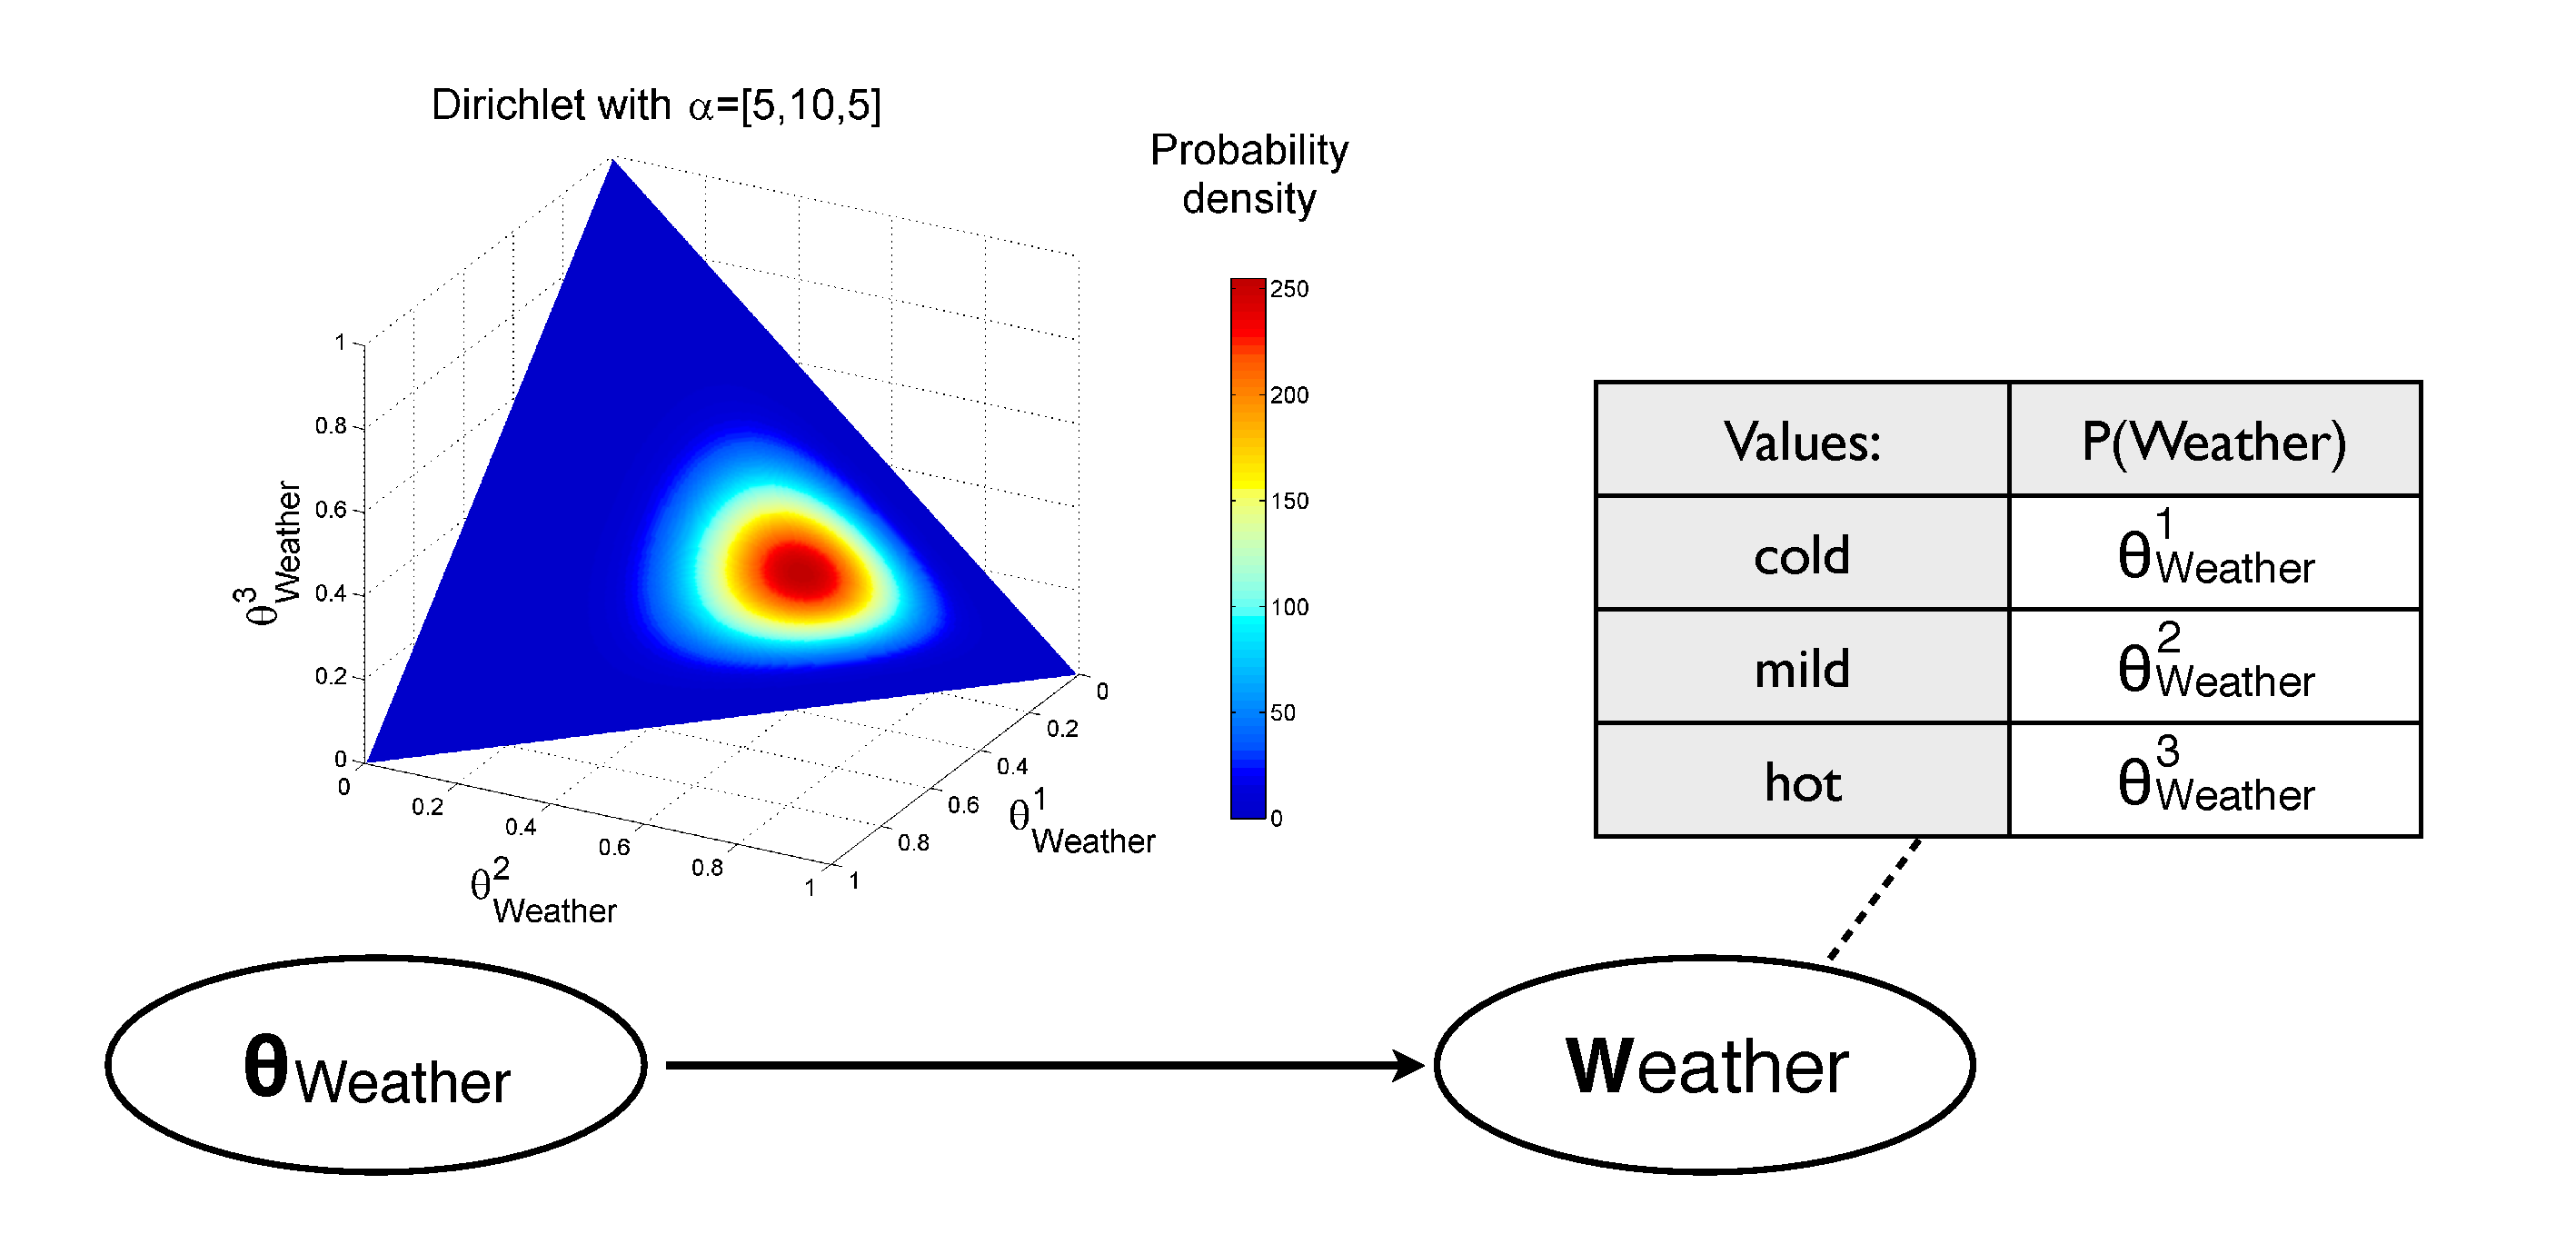
\includegraphics[scale=0.28]{imgs/bayesianlearning.pdf}
\caption{Bayesian network with variable $\mathit{Weather}$ and associated parameter $\theta_{Weather}$.  As $\mathit{Weather}$ is a categorical distribution, the distribution $P(\theta_{Weather})$ is expressed as a Dirichlet with three dimensions that reflect the relative probabilities for the three values in $Val(\mathit{Weather})$. }
\label{fig:baysianlearning}
\end{figure}

In the case of completely observed data, Bayesian learning over several parameters can be decomposed into independent estimation problems (one for each parameter variable): 
\begin{equation}
P(\mathcal{D} \, ; \, \boldsymbol\theta) = \prod_{\theta_i \in \boldsymbol\theta} P(\mathcal{D} \, ; \, \theta_i)
\end{equation}
As in the maximum likelihood estimation case, the learning task becomes more complicated when dealing with partially observed data, as the posterior distribution can no longer be represented as a product of independent posteriors over each parameter.  In this setting, the full posterior is often too complex to be amenable to an analytic solution.  Sampling techniques can however be applied to offer reasonable approximations of this posterior.  As we shall see in Chapter \ref{chap:wozlearning} and \ref{chap:rllearning}, the work presented in this thesis is directly grounded in such approximate Bayesian learning methods. 

Table \ref{table:gmlearning} briefly summarises the parameter estimation methods discussed in this section.

\begin{table}[h]
\renewcommand{\arraystretch}{1.8}
\setlength{\tabcolsep}{10pt}
\vspace{3mm}
\begin{center}
\begin{tabular}{|p{30mm}||p{42mm}|p{48mm}|} \hline 
\centering \textbf{Training data} & \centering \textbf{Maximum likelihood estimation} &  $\ \ \ \ \ \ \ $ \textbf{Bayesian learning} \\ \hline
\textit{Fully observed} & Maximisation of local $\phantom{aa}$ likelihood functions & Query on local posterior distribution over each parameter \\
\textit{Partially observed (hidden variables)} &  Iterative optimisation of global likelihood function &  Query on full posterior over parameters via sampling \vspace{2mm} \\  \hline
\end{tabular}
\end{center}
\caption{Summary of parameter estimation approaches for directed graphical models.}
\label{table:gmlearning}
\end{table}


\section{Reinforcement learning}
\label{sec:rl}

Dialogue management is fundamentally a problem of sequential decision-making under uncertainty. The objective of the dialogue system is to select the action that is expected to be ``optimal'' -- that is, that yields the maximum long-term utility for the agent. However, in many domains (including dialogue domains), the agent has no knowledge of the internal dynamics of the environment it finds itself in.  It must therefore determine the best action to execute in any given state via a process of trial and error.  Such learning process is called \textit{reinforcement learning} (RL).  It is worth noting that reinforcement learning effectively strikes a middle ground between supervised and unsupervised learning.  Contrary to supervised learning, the framework does not require the provision of ``gold standard'' examples.  However,  thanks to the reward function it receives from the environment, the agent is able to get a sense of the quality of its own decisions, an element which is absent in unsupervised learning methods.  

We provide here a brief introduction to the central concepts in reinforcement learning, and refer the interested reader to \cite{citeulike:112017} for more details. 

\subsection{Markov Decision Processes}
\label{sec:mdp}

Reinforcement learning tasks are typically based on the definition of a \textit{Markov Decision Process} (MDP), which is a tuple $\langle \mathcal{S}, \mathcal{A}, T, R \rangle$ where:
\begin{itemize}
\item $\mathcal{S}$ is the state space of the domain and represents the set of all (mutually exclusive) states.
\item $\mathcal{A}$ is the action space and represents the possible actions that can be executed by the agent.
\item $T: \mathcal{S} \times \mathcal{A} \times \mathcal{S} \rightarrow [0,1]$ is the transition function and encodes the probability $P(s'|s,a)$ of reaching state $s'$ after executing action $a$ in state $s$.
\item $R:  \mathcal{S} \times \mathcal{A} \rightarrow \Re$ is the reward value associated with the execution of action $a$ in state $s$.
%\item $s_0 \in \mathcal{S}$ is the initial state of the process.
\end{itemize}
 
Markov Decision Processes can be explicitly represented as dynamic decision networks.  As we can see from the graphical illustration in Figure \ref{fig:mdp}, the state at time $t+1$ is dependent both on the previous state at time $t$ and the action $a_t$ performed by the system. After each action, the system received a reward $r_t = R(s_t, a_t)$ that depends both on the state and selected action. 

\begin{figure}[h]
$\phantom{d}$\hspace{20mm}
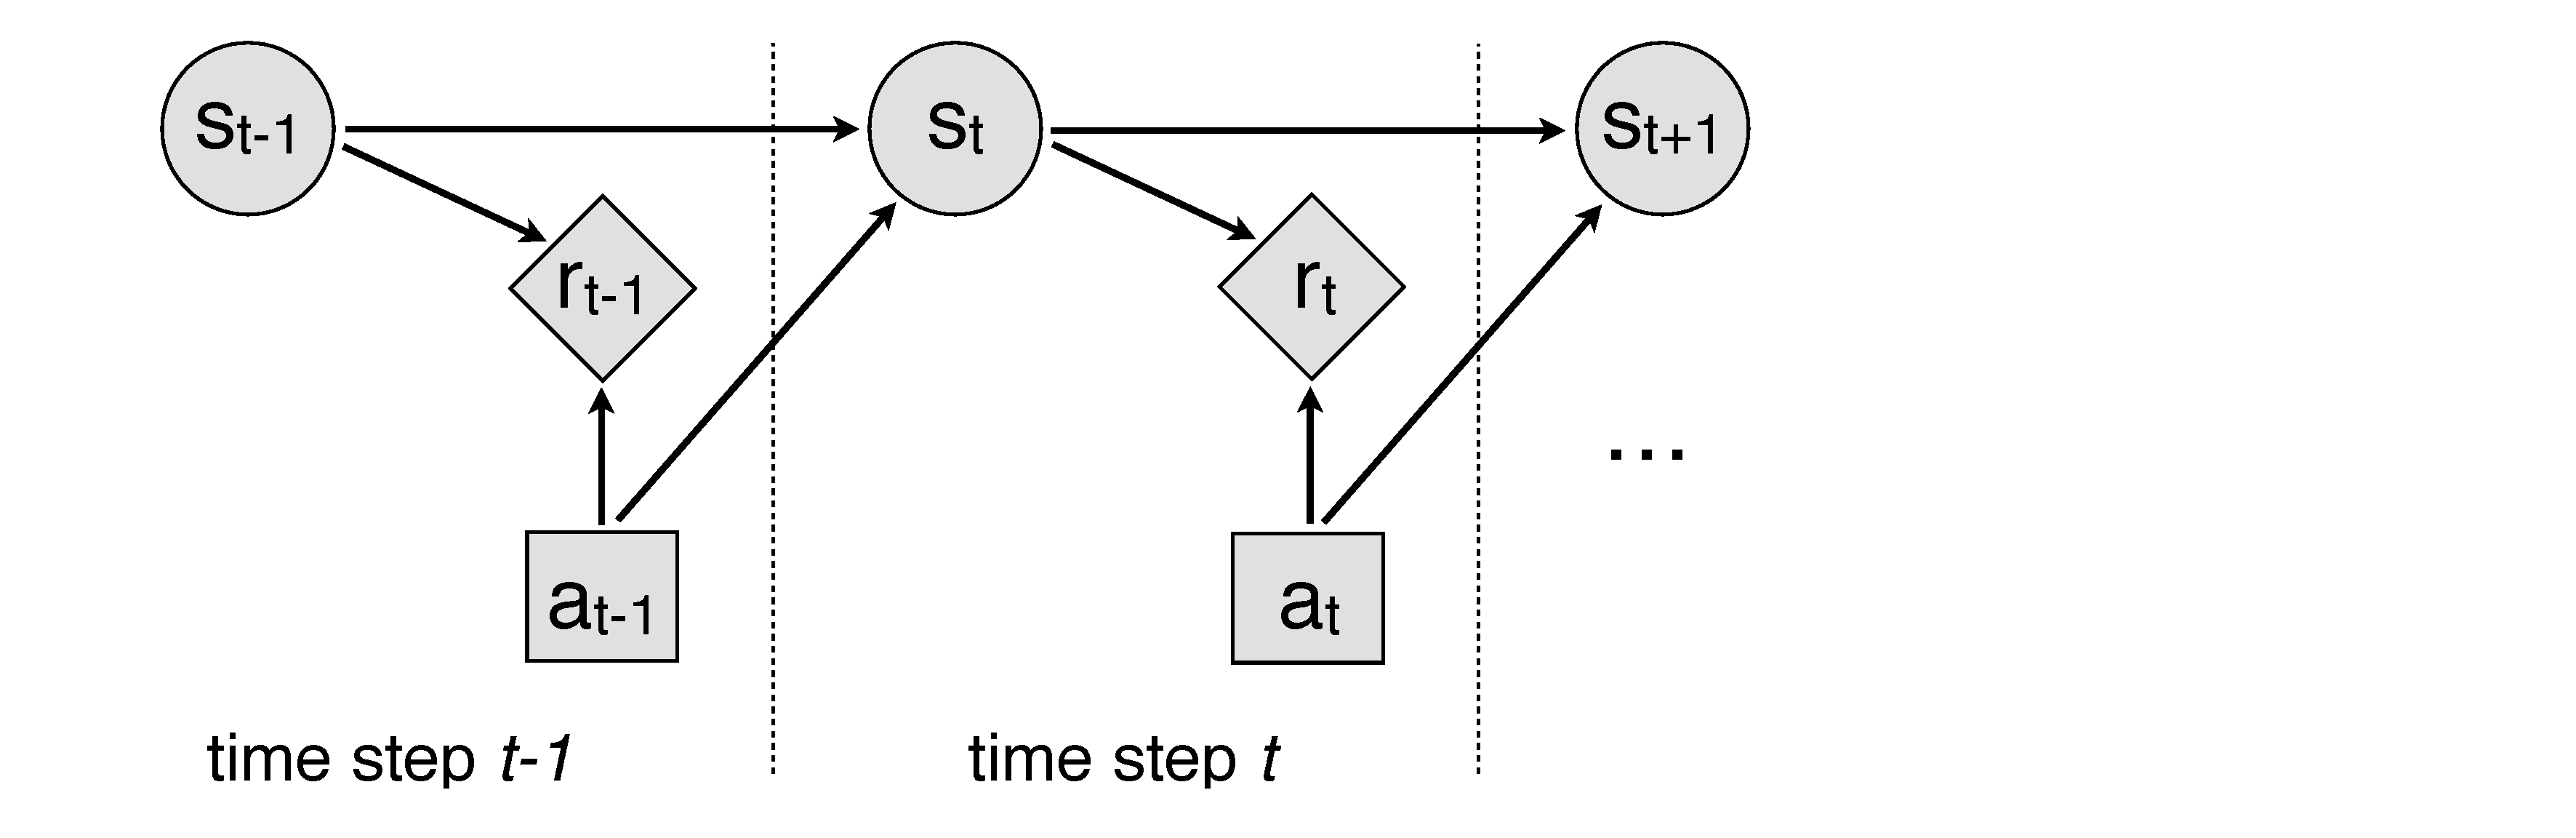
\includegraphics[scale=0.25]{imgs/MDP.pdf}
\caption{Graphical model of a Markov Decision Process (MDP) unfolded on a few time steps.  Greyed entities indicate observed variables. In the MDP case, all past states, actions and rewards are observed, as well as the current state.}
\label{fig:mdp}
\end{figure}

Given a particular MDP problem, the goal of the learning agent is to find an optimal policy $\pi^*: \mathcal{S} \rightarrow \mathcal{A}$ that maps each possible state to the best action to execute at that state.  The best action is the action that maximises the \textit{expected return} for that state, which is the discounted sum of rewards, starting from the current state up to a potentially infinite horizon.  In this sum, a geometric discount factor $\gamma$ (with $0 \leq \gamma \leq 1$) indicates the relative worth of future rewards in regard to present ones. At one extreme, $\gamma = 0$ corresponds to a short-sighted agent only interested in its immediate reward, while $\gamma=1$ corresponds to an agent for which immediate and distant rewards are valued equally. For a given policy $\pi$, the expected return for an arbitrary state $s$ in $\mathcal{S}$ is expressed through the value function $V^{\pi}(s)$:
\begin{align}
V^{\pi}(s) & = \  E \left\{ r_0 + \gamma r_1 + \gamma^2 r_2 + ... \ \big| \ s_0 = s, \pi \text{ is followed} \right\} \\
& = E \left\{\sum_{i=0}^{\infty}  \gamma^i r_{i} \ \bigg| \ s_0 = s, \pi \text{ is followed} \right\} \label{eq:value}
\end{align} 
where $r_i = R(s_i, \pi(s_i))$ is the reward received at time $i$ after performing the action specified by the policy $\pi$  in state $s_i$.  Equation \eqref{eq:value}  can be rewritten in a recursive form, leading to the well-known Bellman equation \citep{Bellman:1957}:
\begin{align}
V^{\pi}(s) & = \    R(s, \pi(s)) + \gamma  \sum_{s' \in \mathcal{S}} P(s'|s,\pi(s)) V^{\pi}(s') \label{eq:bellman}
\end{align} 
In other words, the expected return in state $s$ equals its immediate reward plus the expected return of its successor state.  The recursive definition offered by the Bellman equation is crucial for many reinforcement learning methods, since it allows the value function to be estimated by an iterative process in which the value function is gradually refined until convergence.

Another useful concept is the action-value function $Q^{\pi}(s,a)$ that expresses the return expected after performing action $a$ in state $s$ and following the policy $\pi$ afterwards:
\begin{equation}
Q^{\pi}(s,a) = R(s,a) + \gamma  \sum_{s' \in \mathcal{S}} P(s'|s,a) V^{\pi}(s')
\end{equation}

The value and action-value functions are closely related, as $V^{\pi}(s) = Q^{\pi}(s,\pi(s))$.

The objective of the learning process is to find a policy $\pi^*: \mathcal{S} \rightarrow \mathcal{A}$ which selects the action with highest expected return for all possible states: $V^{\pi^*}(s) \geq V^{\pi}(s)$ for any state $s$ and policy $\pi$.  For a given MDP, there is at least one policy that satisfies this constraint. The value and action-value functions for this optimal policy are respectively denoted $V^*$ and $Q^*$. 

Two families of reinforcement learning approaches can be used to determine this policy: \begin{enumerate}
\item  \textit{Model-based} approaches first estimate an explicit model of the MDP and subsequently optimise a policy based on this model. The agent initially collects data by interacting with its environment and recording the reward and successor state following each action. Based on this data, standard parameter estimation methods (as outlined in Section \ref{sec:learning}) can be used to fix the MDP parameters, and the resulting model is  applied to extract the corresponding optimal policy via dynamic programming \citep{Bertsekas:1996} or more advanced Bayesian methods \citep{DeardenFA99}.  The most well-known model-based learning algorithm is \textit{value iteration}, which operates by estimating the value function via a sequence of updates based on Bellman's equation. Given a value function estimate $V_k$ available at step $k$, the estimate at step $k+1$ is calculated as: 
\begin{equation}
V_{k+1}(s) = \max_a R(s,a) + \gamma \sum_{s' \in \mathcal{S}} P(s' \, | \, s, a) \ V_k(s')
\end{equation}

Once the iterations have converged, the optimal policy is straightforwardly derived as:
\begin{equation}
\pi^*(s) = \argmax_a Q^*(s,a)
\end{equation}

\item \textit{Model-free} approaches skip the estimation of the underlying MDP model in order to directly learn $Q^*$ functions from the agent's interaction experience.  The most popular model-free techniques are Q-learning \citep{watkins92}, SARSA \citep{rummery:phd95} and gradient descent \citep{Sutton:2009}.  The main idea behind model-free methods is to let the agent try out different actions, observe the effects in terms of rewards and successor state, and use this information to refine the estimate of the $Q^*$ function. This operation is repeated for a large number of episodes until convergence.  
\end{enumerate}

One key question that must be addressed in both model-based and model-free approaches is how  to efficiently explore the space of possible actions.  The agent should indeed favour the selection of high-utility actions in most cases (since they are the ones of interest to the agent), but should also occasionally explore actions that are currently thought to be less effective to avoid being stuck in a suboptimal behaviour. This trade-off, called the \textit{exploration-exploitation} dilemma, is one of the central research questions in reinforcement learning. 


\subsection{Partially Observable Markov Decision Processes}
\label{sec:pomdp}

A limitation faced by MDP approaches is the assumption that the dialogue state is fully observable. As we already noted in the previous chapter, this assumption does not hold for most dialogue systems, owing to the presence of multiple sources of uncertainty, due in particular to speech recognition errors.  An elegant solution to this problem is to extend the MDP framework by allowing the state to be a hidden variable that is indirectly inferred from observations.  Such extension gives rise to a  \textit{Partially Observable Markov Decision Process} (POMDP).  POMDPs are formally defined as tuples $\langle \mathcal{S}, \mathcal{A}, T, R, \mathcal{O}, Z \rangle$.  As in a classical MDP, $\mathcal{S}$ represents the state space, $\mathcal{A}$ the action space, $T$ the transition probability $P(s'|s,a)$ between states, and $R$ the reward function $R(s,a)$.  However, the actual state is no longer directly observable.  Instead, the process is associated with an observation space $\mathcal{O}$ that expresses the set of possible observations that can be perceived by the system. The function $Z$ then defines the probability $P(o|s)$ of observing $o$ in the current state $s$.  Figure \ref{fig:pomdp} provides a graphical illustration of the POMDP framework.  As we can see, POMDPs can also be expressed as dynamic decision networks in which the state variable is not directly observed. 

\begin{figure}[h]
\centering
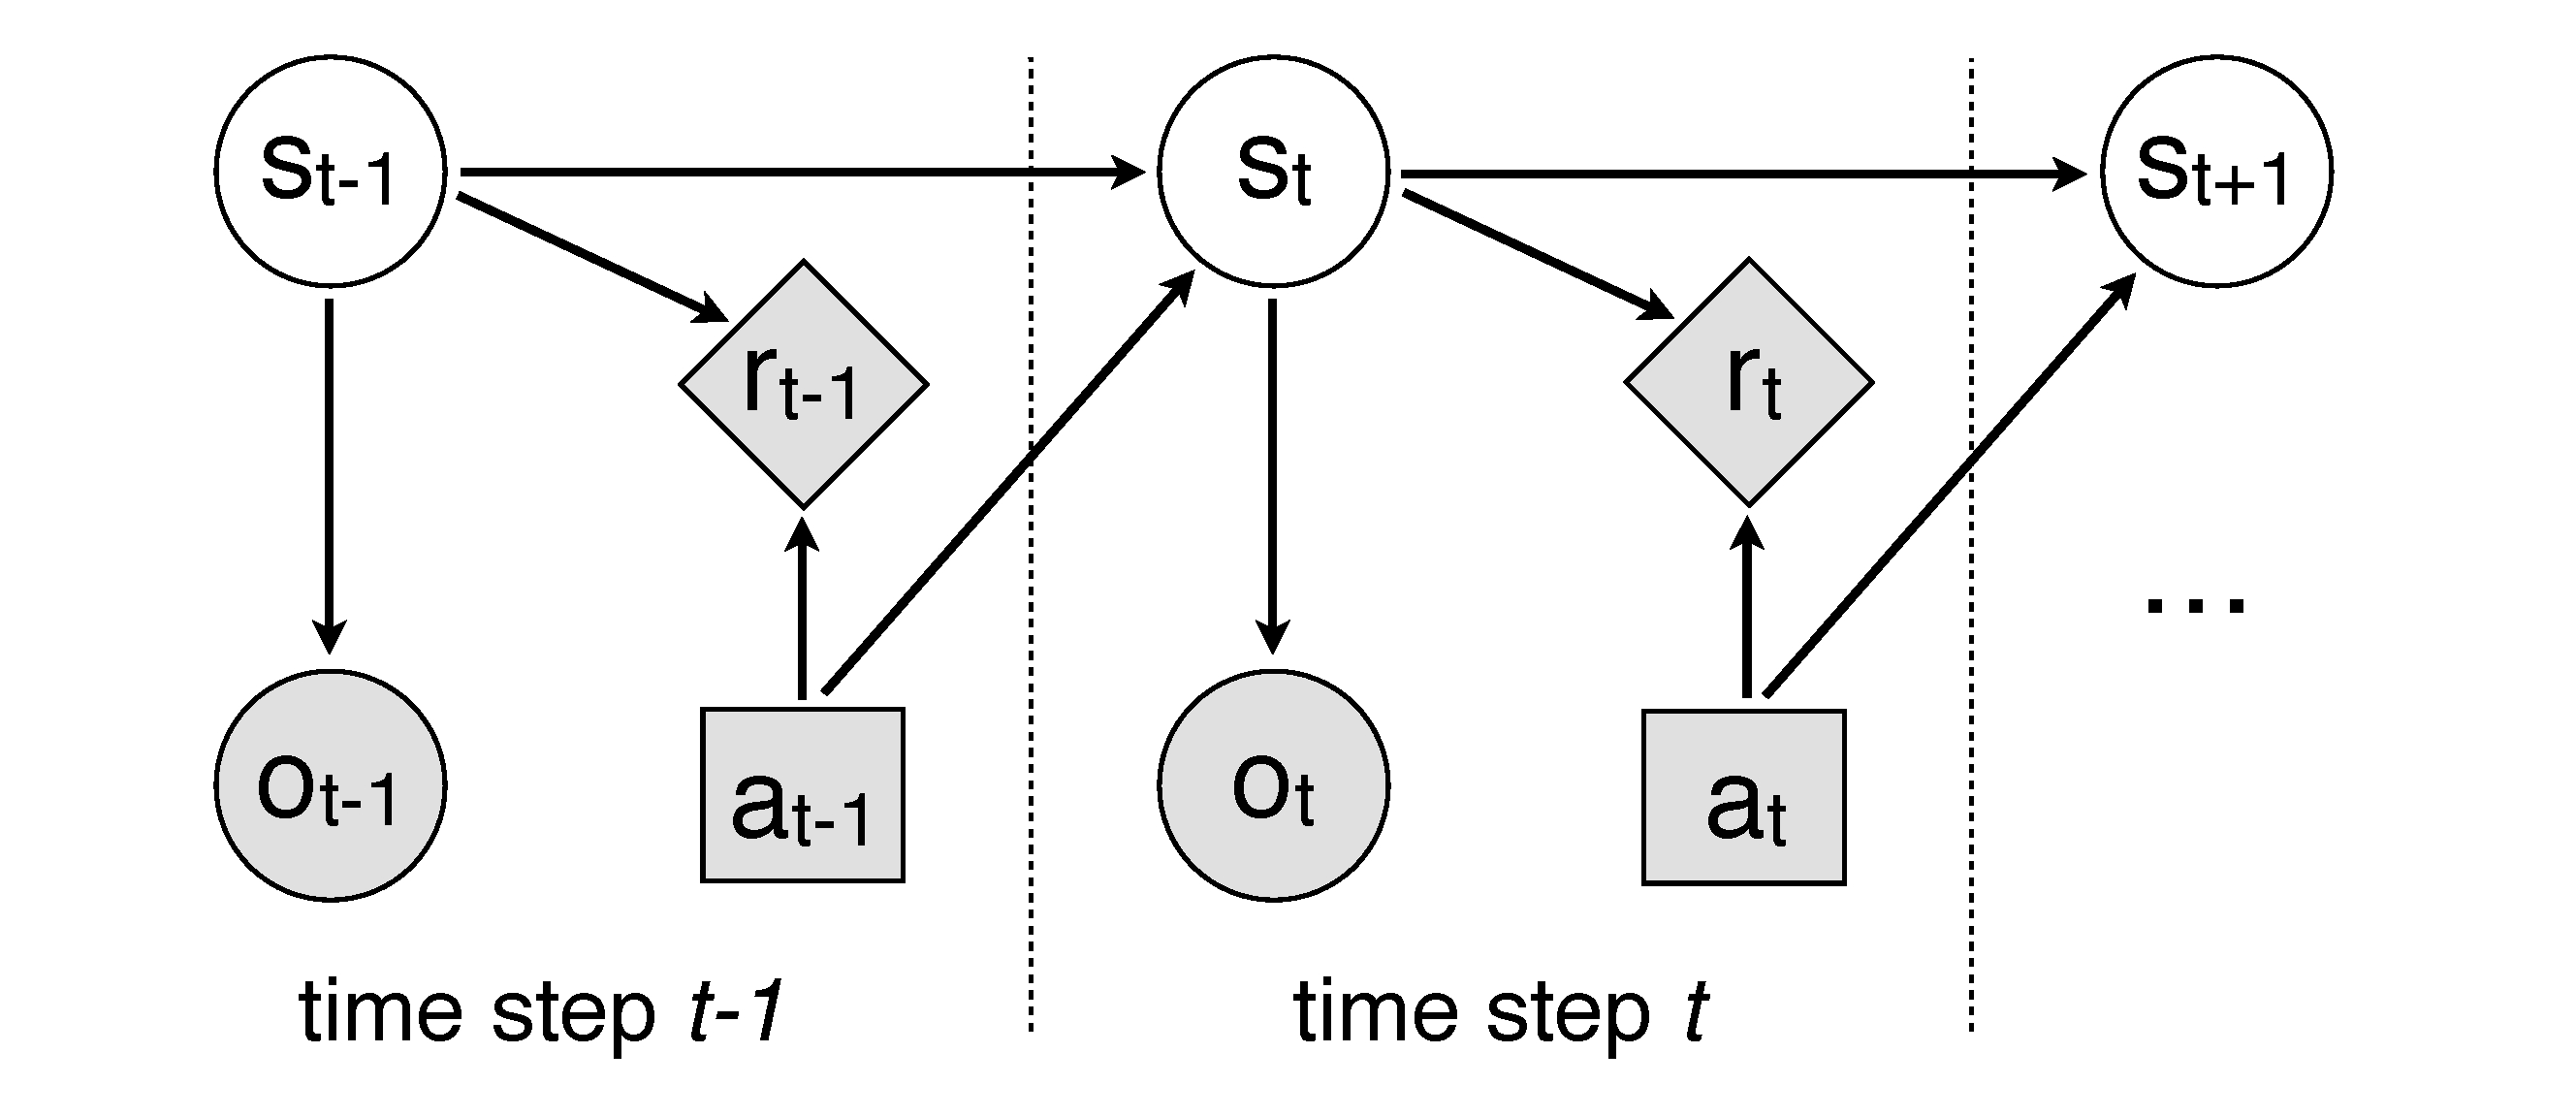
\includegraphics[scale=0.25]{imgs/POMDP.pdf}
\caption{Graphical model of a Partially Observable Markov Decision Process (POMDP) unfolded on a few time steps.  Compared to Figure \ref{fig:mdp}, we notice that the state is no longer directly accessible but must be inferred from the observations and (predicted) state history. }
\label{fig:pomdp}
\end{figure}

The agent knowledge at a given time is represented by the \textit{belief state} $b$, which is a probability distribution $P(s)$ over possible states.  After each system action $a$ and subsequent observation $o$, the belief state $b$ is updated to $b'$ in order to incorporate the new information.  This belief update is a simple application of Bayes' theorem: 
\begin{align}
b'(s) = \ \!P(s'|b, a,o) & = \ \frac{P(o|s') \ P(s'|b,a)}{P(o|b,a)} \\[3mm]
& = \eta \ P(o|s') \sum_{s} P(s'|s,a) \ b(s) \label{eq:update}
\end{align}
where $\eta = P(o|b,a)$ serves as a normalisation constant and is usually never calculated explicitly. 

In the POMDP setting, a policy is a function $\pi = \mathcal{B} \rightarrow \mathcal{A}$ mapping each possible belief state to its optimal action.  Mathematically, the belief state space $\mathcal{B}$ is a $(|\mathcal{S}|\!-\!1)$-dimensional simplex (where $|\mathcal{S}|$ is the size of the state space), which is a continuous and high-dimensional space. The optimisation of the dialogue policy is therefore considerably more complex than for MDPs. The value function $V^{\pi}$ for a policy $\pi$ is the fixed point of Bellman's equation: 
\begin{equation}
V^{\pi}(b) = \sum_{s \in S} \ R(s,a) b(s) + \gamma \sum_{o \in \mathcal{O}} P(o|b,\pi(b)) \ V^{\pi}(b')
\end{equation}
where $b'$ is the updated belief state following the execution of action $\pi(b)$ and the observation of $o$, as in Equation \eqref{eq:update}.  The optimal value function $V^*(b)$ for finite-horizon problems is known to be piecewise linear and convex in belief space, as proved by \cite{Sondik1971}. The value function can therefore be represented by a finite set of vectors, called $\alpha$-vectors. Each vector $\alpha_i$ is associated with a specific action $a(i) \in \mathcal{A}$.\footnote{Note that the reverse is not true: each action can be associated with an arbitrary number of vectors.}  The vectors are of size $|\mathcal{S}|$ and $\alpha_i(s)$ is a scalar value representing the value of action $a(i)$ in state $s$.  Given these vectors, the value function simplifies to:
\begin{equation}
V^*(b) = \max_{i} \alpha_i \cdot b
\end{equation}
And the policy $\pi^*$ can be rewritten as:
\begin{equation}
\pi^*(b) = a\left(\argmax_i(\alpha_i \cdot b)\right)
\end{equation}

Extracting the $\alpha$-vectors associated with a POMDP problem is however computationally challenging given the high-dimensional and continuous nature of the belief space, and exact solutions are intractable beyond toy domains. As shown by \cite{Papadimitriou:1987}, deriving the $\alpha$-vectors for a given POMDP -- also known as ``solving'' the POMDP -- is a PSPACE-complete problem, which means that the best known algorithms will take time $2^{poly(n,h)}$ to solve a problem with $n$ states and a planning horizon $h$.

A number of approximate solutions have however been developed.  One simple strategy is to rewrite the $Q(b,a)$ function in terms of the $Q$-values for the underlying MDP, as described by \cite{Littman:1997}:
\begin{equation}
Q(b,a) = \sum_{s \in \mathcal{S}} Q_{MDP} (s,a) b(s)
\end{equation}
Although this approximation can work well in some settings, it essentially rests on the assumption that the state uncertainty will disappear after one action.  It is therefore a poor model for information-gathering actions -- that is, actions that do not change the actual state but might help in reducing state uncertainty.\footnote{A typical example of such action in dialogue is a clarification request about the user intention.} 

Many approximations methods focus on simplifying the belief state space, notably through the use of grid-based approximations \citep{Zhou:2001}.  The idea is to estimate the value function only at particular points within the belief simplex. At runtime, the action-value function for the current belief state $b$ is then approximated to the value for the closest point in the grid according to some distance measure. Instead of using a fixed grid, most recent solution methods rely on sampling techniques to perform local value updates at specific belief points \citep{Pineau_2003,KurHsu08}. Belief compression has also proved to be useful \citep{Roy:2005}.  Yet another family of optimisation methods directly search in the space of possible policies constrained to a particular form such as finite-state controllers \citep{Hansen98}. 

A final alternative, which we follow in Chapter \ref{chap:rllearning} of this thesis, is to rely on online planning algorithms \citep{ross2008,NIPS2010_0740}.  The idea is to let the agent estimate the $Q(b,a)$ values at execution time via look-ahead search on a limited planning horizon. Compared to offline policies, the major advantage of online approaches is that the agent only needs to consider the current state to plan instead of enumerating all possible ones. It can also more easily adapt to changes in the reward or transition models, as the policy is not compiled in advance but generated at runtime. Online planning can moreover be used to simultaneously learn or refine these models during the interaction, as demonstrated by \cite{Ross:2011}.  The available planning time is however more limited, since planning is in this case interleaved with system execution and must therefore meet real-time constraints. %Section \ref{sec:online-planning} presents an anytime planning algorithm for probabilistic rules. 

Despite these recent advances, the optimisation of POMDP policies remains nevertheless to a large extent an open research question in the fields of reinforcement learning and decision-theoretic planning. One important insight that transpires in much of the POMDP literature is the importance of exploiting the problem structure to reduce the complexity of the learning and planning problems \citep{Pineau:2004,poupart2005}.  As detailed in the next chapter, the work presented in this thesis precisely attempts to transfer this insight into dialogue management. 

\subsection{Factored representations}
\label{sec:factored}

In the previous pages, we modelled the system states and actions as atomic symbols.  Such plain representations can unfortunately quickly lead to a combinatorial explosion of the state-action spaces. A more efficient alternative is to apply \textit{factored} representations that decompose the state into distinct variables with possible conditional dependencies between one another.  Similarly, action variables can also be split into distinct variables.  For a MDP, the state will take the form of a set of variables $\mathbf{S}_t$, and the transition function $P(\mathbf{S}_t \, | \, \mathbf{S}_{t-1},\mathbf{A}_{t-1})$ be represented as a dynamic Bayesian network \citep{boutilier1999}. The reward function can also be encoded as a collection of utility variables $\mathbf{R}_t$ connected to relevant sets of state and action variables. In such case, the total utility is defined as the sum of all utilities.

POMDPs can be factored in a similar way, with the inclusion of observation variables $\mathbf{O}_t$ connected to the state variables $\mathbf{S}_t$ through conditional dependencies $P(\mathbf{O}_t \, | \, \mathbf{S}_t)$.  At time $t$, the observation variables $\mathbf{O}_t$ will be observed while the state variables  $\mathbf{S}_t$ remain hidden. Figure \ref{fig:pomdp3} illustrates this factorisation. Both plain and factored (PO)MDPs form specific cases of dynamic decision networks, as illustrated in the figure.

\begin{figure}[h]
\centering
\includegraphics[scale=0.25]{imgs/pomdp3.pdf}
\caption{Factored representation of a POMDP with state variables $\mathbf{S}$, action variables $\mathbf{A}$, observations variables $\mathbf{O}$, and reward variables $\mathbf{R}$. }
\label{fig:pomdp3}
\end{figure}

\section{Application to dialogue management}
\label{sec:application-dm}

We have now reviewed the key ideas of probabilistic reasoning and reinforcement learning, and are ready to explain how these ideas can be practically transferred to the dialogue management task.  After a brief review of supervised learning approaches, we detail how dialogue can be modelled as a Markov Decision Process or Partially Observable Markov Decision Process, and survey the various optimisation techniques that have been developed to automatically optimise dialogue policies for such models based on real or simulated interaction data.  

\subsection{Supervised learning from Wizard-of-Oz data}

The most straightforward use of statistical approaches to dialogue management is to learn dialogue policies in a supervised learning manner, based on collected  Wizard-of-Oz data where dialogue management is remotely performed by a human expert.  The resulting training data is a sequence $\{( s_i, a_i ) : 1 \leq i \leq n\}$ of state-action pairs, where $s_i$ is the state at time $i$ and $a_i$ the corresponding wizard action, which is assumed to reflect the best action to perform in this state.  Most supervised learning approaches encode the dialogue state as a list of feature-value pairs, and the goal of the learning algorithm is to train a classifier $C: \mathcal{S} \rightarrow \mathcal{A}$  from state to actions that produces the best fit for this training data (modulo regularisation constraints), and will therefore ``mimic'' the decisions of the wizard in similar situations. Various classifiers can be used for this purpose, such as maximum likelihood classification \citep{Hurtado:2005}, decision trees \citep{LaneKU04}, Naive Bayes \citep{williams2003}, and logistic regression \citep{rieser2006,Passonneau2012}.  

One important issue in supervised learning approaches is data sparsity, as only a fraction of the possible states can realistically be covered by the Wizard-of-Oz interactions.  Several generalisation techniques can be employed to alleviate this problem.  The simplest is to encode in a parametric form in which the parameters are associated with a smaller number of features extracted from the state-action pair. The size of the feature set can be further reduced with feature selection \citep{Passonneau2012}. Yet another approach put forward by \cite{Hurtado:2005} is to couple the classifier with a distance measure between states, thereby allowing the reuse of strategies learned from closely related states.

% note about our approach: generalisation enable a better account of the data sparsity problem.  plus, the state dynamics are not lost since we perform belief update.  Finally, the appraoch can be seen as an initial boostrapping that can then be further refined through online reinforcement learning (Bayesian prior), as in Williams etc. also, we learn utilities, not a direct classification. Also: a user simulator is difficulty for situated and open-ended environments.  we learn a POMDP policy by simulation

\subsection{MDP-based optimisation of dialogue policies}

Instead of learning a dialogue policy by imitating the behaviour of human experts, the dialogue manger can also learn by itself the best action to perform in each possible conversational situation via repeated interactions with a (real or simulated) user.  Dialogue management can indeed be cast as a type of Markov Decision Process $\langle \mathcal{S}, \mathcal{A}, T, R \rangle$ in which: 
\begin{itemize}
\item The state space $\mathcal{S}$ corresponds the set of possible dialogue states, usually encoded as a list of feature-value pairs that capture relevant aspects of the current conversational context.
\item The actions space $\mathcal{A}$ corresponds to the set of (verbal or extra-verbal) actions that can be executed by the system.
\item The transition function $T$ captures the ``dynamics'' of the conversation, and indicates how the dialogue state is expected to change as a result of the system actions (and in particular how the user is expected to respond). 
\item The reward function $R$ expresses the objectives and costs of the application. A common reward function is to assign a high positive value for the successful completion of the task, a high negative value for a failure, and a small negative value for soliciting the user to repeat or clarify her/his intention.  
\end{itemize}

A common misunderstanding should be clarified at this point. The representation of dialogue as a Markov Decision Process implies that the transition function only considers the previous state and action to predict the next state.  It has occasionally been argued in the literature that this formalisation makes the decision-making process oblivious to non-local aspects of the dialogue history. This argument is however invalid, as the dialogue state is not limited to the mere representation of the last dialogue act but may express any features related to the interaction context, including variables recording dialogue histories of arbitrary length, long-term user intentions, and so forth.  It is ultimately up to the system designer to decide which features are deemed relevant to describe the current state of the dialogue. 

\subsubsection*{Dialogue state representation}

As for supervised learning methods, MDP-based reinforcement learning approaches to dialogue management encode the dialogue state in terms of feature-value pairs.  The dialogue state is thus factored into a number of independent variables (one for each feature).  Most early approaches adopted crude state representations with features limited to the status of the slots to fill and the last user utterance \citep{817450,Singh:2000:EER:647288.723412,Scheffler:2002}.  The voice-enabled email client described in \cite{Walker:2000} captured additional measures related to the overall task progress, history of previous system attempts, confidence thresholds and timing information.  There has also been some work on the automatic identification of relevant state variables, using methods from structure learning in decision networks \citep{PaekC06} and feature selection \citep{tetreault2006using}. 

\cite{Henderson:2008} are to our knowledge the first to explore the extension of reinforcement learning methods to large state spaces based on rich representations of the conversational context. Inspired by information state approaches to dialogue management, their state space captures detailed information such as complete history of dialogue acts and fine-grained representations of the task status, amounting to a total of $10^{386}$ possible states.  Such rich state representations allow the dialogue manager to exploit much broader contextual knowledge in its decision-making.  However, it also creates important challenges regarding action selection, as generalisation techniques are necessary to scale up the learning procedure to such large state spaces.
'
\subsubsection{Policy optimisation (and associated generalisation techniques)}

For most dialogue domains, the reward is fixed in advance by the system designer and reflects the task objectives.  It can also correspond to a performance metric such as \textsc{Paradise} \citep{Walker:2000}.  The metric is defined in such case as a linear combination of quantitative measures whose weight is empirically estimated via multivariate linear regression from surveys of user satisfaction.\footnote{Quantitative measures of dialogue performance are typically classified in three categories: \textit{task success} (e.g. ratio of successfully completed vs. failed tasks, $\kappa$ agreement for slot-filling applications), \textit{dialogue quality} measures (e.g. number of repetitions, barge-ins, ASR rejection prompts) and \textit{dialogue efficiency} measures (e.g. number of utterances per dialogue, total elapsed time).}

The transition probabilities are however typically unknown.  As described in Section \ref{sec:mdp}, two families of approaches can be followed to optimise dialogue policies: model-based approaches first learn an explicit model of the MDP from interaction data and then extract a policy for this model, while model-free approaches directly estimate an action-value function $Q^*(s,a)$ from interactions, without explicit model of the state transitions.  

While it is possible to follow a model-based strategy and learn explicit distributions for the transition probabilities \citep{SinghLKW02,tetreault2006using}, the majority of recent RL approaches to dialogue management have adopted model-free techniques. Due to the significant amounts of data necessary to reach convergence, it is often impossible to directly learn the value function from interactions with real users for most practical domains.  A user simulator is instead used to provide unlimited supplies of interactions to the reinforcement learning algorithm.   Several options are available to construct this user simulator.  The first option is to design it manually based on specific assumptions about the user behaviour \citep{Pietquin:2006,Schatzmann:2007:AUS:1614108.1614146}.  It can also be constructed in a data-driven manner from existing corpora \citep{GeorgilaHL06}.\footnote{The most important corpus of human-machine dialogue is the \begin{small}\textsc{Communicator}\end{small} dataset of telephone conversations in the domain of travel planning, with more than 180,000 utterances (90 hours of recording) transcribed and annotated with various understanding and dialogue-level information \citep{BennettR02}.}  In such case, user simulation can be interpreted as a way to expand the initial data set.  The third available option is to exploit  Wizard-of-Oz studies to tune the simulator parameters \citep{Rieser:2010:LHM:1735495.1735497}.  In addition to user modelling, the simulator should also integrate error modelling techniques in order to simulate various types of errors that may appear along the speech recognition and understanding pipeline \citep{SchatzmannTY07,ThomsonGHTY12}

The key benefit of user simulation lies in the possibility to explore a large number of possible dialogue trajectories and error types.  Such simulation is in particular of great use for prototyping dialogue policies and experimenting with alternative setups. However, simulated interactions are not as valuable as real interactions, and offer no guarantee of matching the behaviour and error patterns of actual users.  The practice of evaluating the performance of dialogue policies based on the same simulator as the one used for training has also been put into question \citep{paek2006}

A key problem in reinforcement learning methods is the \textit{curse of dimensionality}: the number of parameters grows exponentially with the size of the state and action spaces \citep{citeulike:112017}.  In order to scale the learning procedure to larger and more complex domains, factorisation and generalisation techniques are often necessary.  An early example of this line of research is the work of \cite{PaekC06} on the use of graphical models in dialogue policy optimisation. The dialogue domain used in their experiments was a speech-enabled web browser.  Their strategy was to explicitly represent the dialogue management task as a dynamic decision network and learn both the structure and parameters of this network from user simulations.  The state space initially included all features that could be automatically logged from the interactions.  Based on the simulated dialogues, the learning algorithm was able to automatically discover the subset of state variables that were relevant for decision-making as well as the transition probabilities between these variables.   They also experimented with various Markov orders to analyse the impact of longer state histories on the system performance.  After the estimation of the decision network, dynamic programming techniques were used to extract a dialogue policy that is optimal with respect to the learned models. Given the complexity of the optimisation, the dynamic programming solution was approximated via forward sampling \citep{Kearns99asparse}. 

\cite{Henderson:2008} demonstrated how to reduce the complexity of model-free learning techniques via function approximation.  As the large size of their state-action space prevented the use of classical tabular representations for the $Q(s,a)$ function, they instead relied on function approximation to define the $Q$-values as a linear function of state features:
\begin{equation}
Q(s,a) = f(s)^{T} w_a 
\end{equation}
where $f(s)$ is a feature vector extracted from the state and $w_a$ a weight vector for action $a$. The weight vectors were learned with the SARSA algorithm based on a fixed corpus (thereby avoiding the use of user simulators). To further refine the estimation of $Q$-values, they also combined estimates from both supervised and reinforcement learning in their final model. 

Hierarchical abstraction is another way to reduce the search space of the optimisation process, as shown by \cite{Heriberto2011}. Instead of viewing action selection as a single monolithic policy, the selection is decomposed in their work into multiple levels, each responsible for a specific decision problem.  This decomposition is formally expressed via an hierarchical extension of MDPs called Semi-Markov Decision Processes.  Each level in the hierarchy is associated with its own subset of state and action variables.  This modular approach allows a complex policy to be split into a sequence of simpler decisions.  Such hierarchical formalisation is particularly natural for task-oriented dialogues, which are known to exhibit rich attentional and intentional structures, as notably argued in the seminal work of \cite{Grosz:1986}. It also bears similarities with the approach presented by \cite{Litman87} on dialogue understanding based on a plan structure. 

Finally, it is worth noting that several researchers have attempted to combine the benefits of supervised and reinforcement learning methods by initialising a RL algorithm with a policy estimated via supervised methods \citep{williams2003, rieser2006}.

\subsection{POMDP-based optimisation of dialogue policies}

To capture the uncertainty associated with many state variables, dialogue can be explicitly modelled as a Partially Observable Markov Decision Process $\langle \mathcal{S}, \mathcal{A}, T, R, \mathcal{O}, Z \rangle$.  Modelling a dialogue domain as a POMDP is similar in most respects to the MDP formalisation.  The observations in $\mathcal{O}$ typically correspond to the possible N-best lists that can be generated by the speech recogniser and NLU modules, and can also include observations perceived via the other modalities.  

\subsubsection*{Dialogue state representation}

POMDP approaches express state uncertainty through the definition of a belief state $b$, which is a probability distribution $P(s)$ over possible states.  After a system action $a$ in belief state $b$ followed by observation $o$, the belief state $b$ is updated according to Equation \eqref{eq:update}, repeated here for convenience:
\begin{align}
b' = P(s'|b, a,o) = \eta \ P(o|s') \sum_{s} P(s'|s,a) \ b(s)   \tag{\ref{eq:update}}
\end{align}

Belief update requires the specification of two probabilistic models: the observation model $P(o|s')$ and the transition model $P(s'|s,a)$. Many POMDP approaches to dialogue management factor the state $s$ into (at least) three distinct variables $s = \langle a_u, i_u, c \rangle$, where $a_u$ is the last user dialogue act, $i_u$ the current user intention(s), and $c$ the interaction context.\footnote{Some approaches also define a specific variable for the dialogue history \citep{Young:2010}.}   Assuming that the observation $o$ only depends on the last user act $a_u$, and that $a_u$ depends on both the user intention $i_u$ and the last system action $a_m$, Equation \eqref{eq:update} is then rewritten as:
\begin{align}
b' & = \ P(a_u', i_u', c' \, | \, b, a_m,o)\\
& = \ \eta \ P(o \, | \, a_u') \ P(a_u' \, | \, i_u', a_m) \sum_{i_u, c'} P(i_u' \, | \, i_u,a_m, c') P(c') \ b(i_u) \label{eq:update2}
\end{align}

The transition model is decomposed in this factorisation into two distinct distributions: \begin{enumerate}
\item  The distribution $P(a_u' \, | \, i_u', a_m)$ is called the \textit{user action model} and defines the probability of a particular user action given her/his underlying intention and the last system act.  It expresses the likelihood of the user action $a_u'$ following the system action $a_m$ and the compatibility of $a_u'$ with the user intention $i_u'$ \citep{Young:2010}.
\item The distribution $P(i_u' \, | \, i_u, a_m, c')$ is the \textit{user goal model} and captures how the user intention is likely to change as a result of the context and system actions.  
\end{enumerate}

These two distributions are usually derived from collected interaction data. A graphical illustration of this state factorisation is shown in Figure \ref{fig:pomdp2}. 

\begin{figure}[h]
\centering
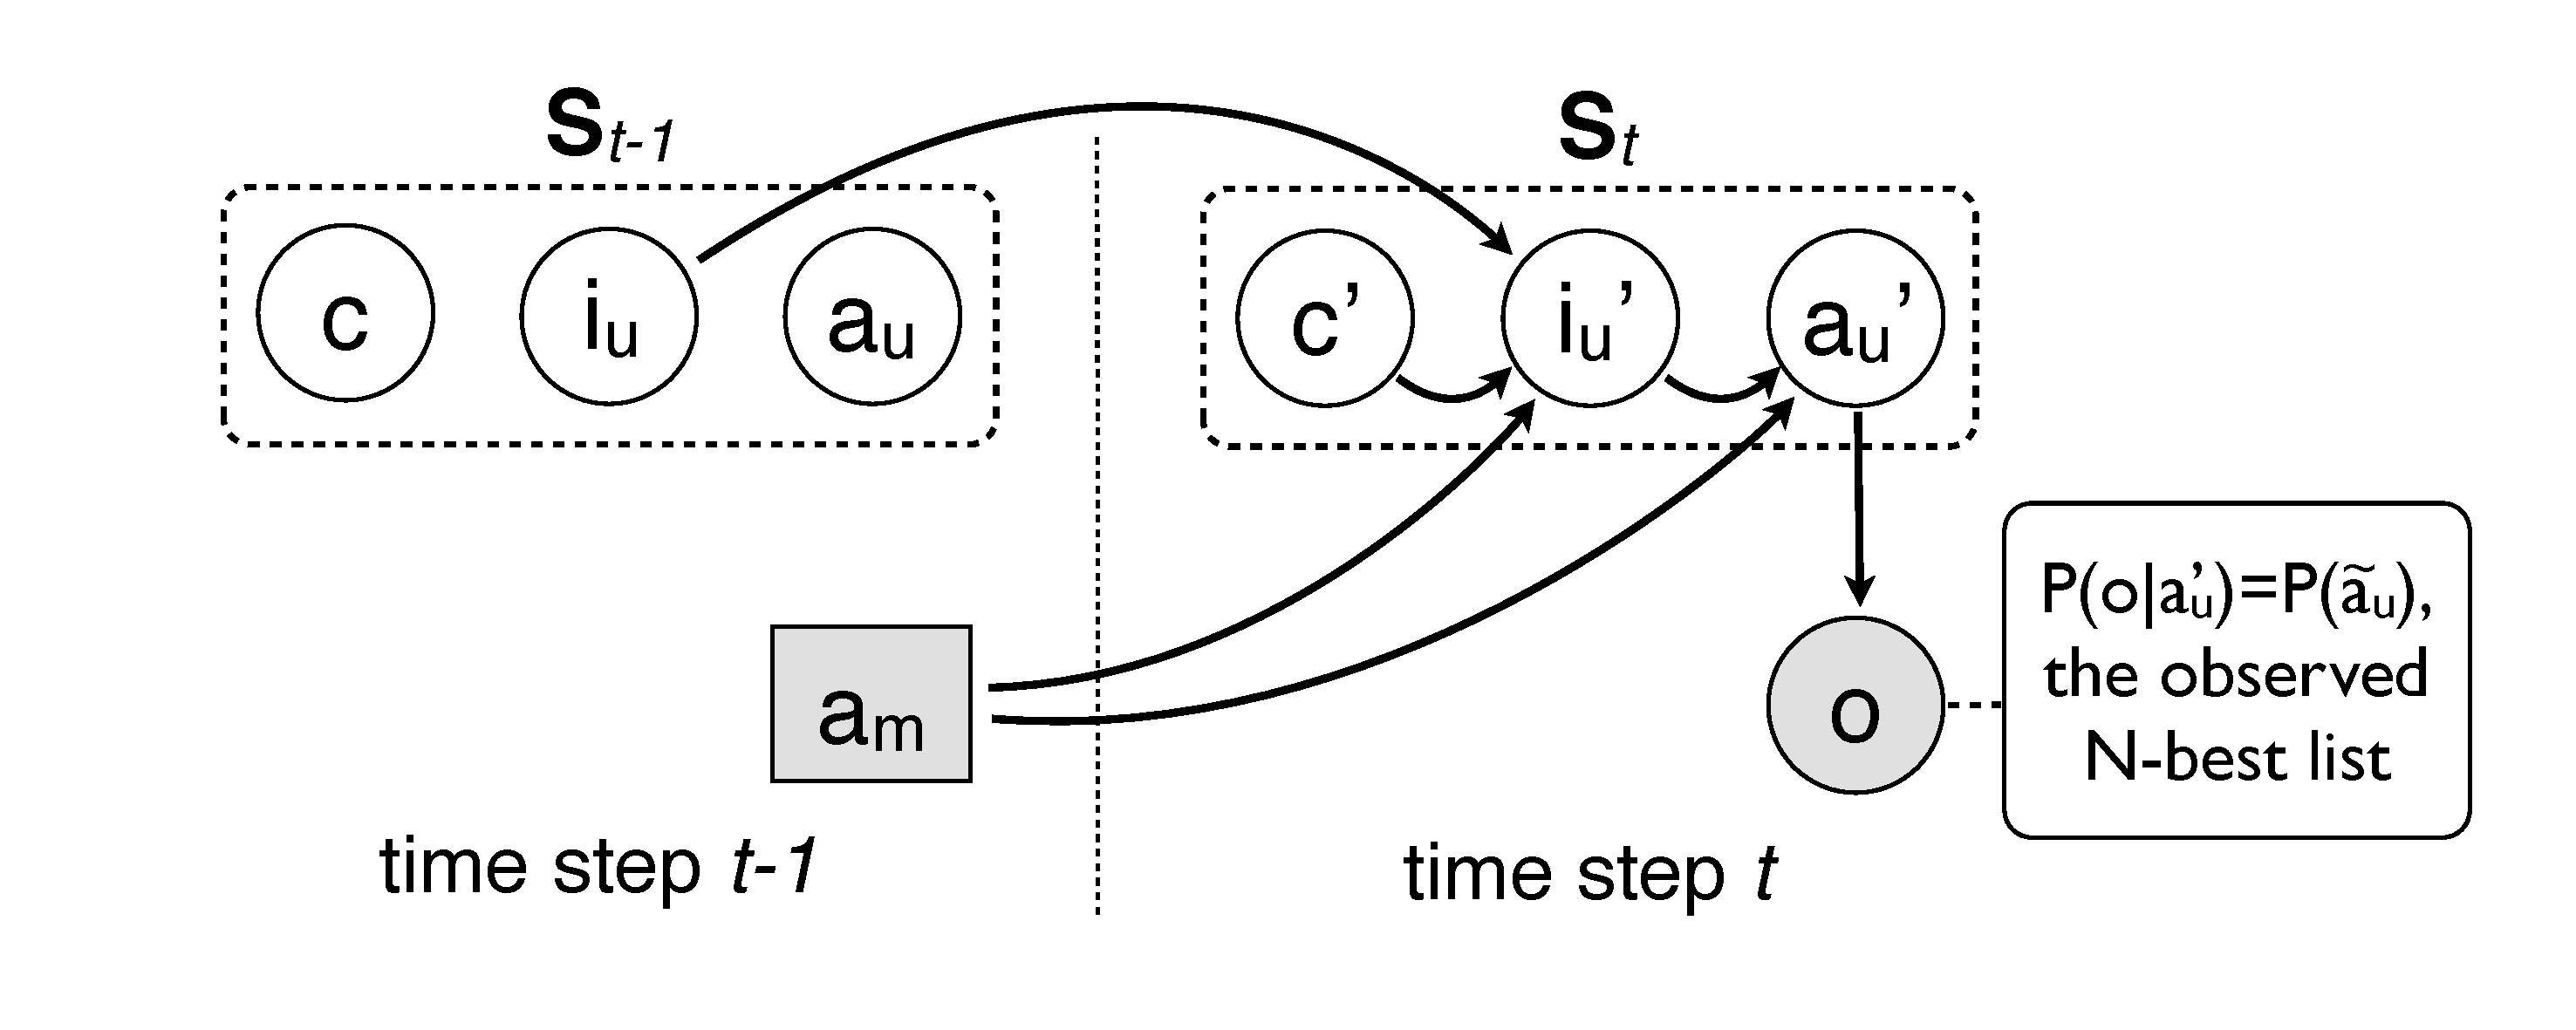
\includegraphics[scale=0.30]{imgs/POMDP2.pdf}
\caption{Common factorisation of the state space for a POMDP-based dialogue system, where $c$ represents the dialogue context, $i_u$ the user intention(s), $a_u$ the user dialogue act, $a_m$ the system act, and $o$ the observed N-best list hypotheses. The representation omits the conditional dependencies and probability distribution for the variable $c'$, which are contingent on the particular interaction context in place for the domain.}
\label{fig:pomdp2}
\end{figure}

The observation model $P(o \, | \, a_u')$ is often rewritten as $P(\tilde{a}_u)$, the dialogue act probability in the N-best list provided by the speech recognition and semantic parsing modules (cf. Section \ref{section:speechunderstanding}), based on the following approximation:
\begin{equation}
P(o \, | \, a_u') = \frac{P(a_u' \, | \, o) \ P(o)} {P(a_u')} \approx P(a_u' \, | \, o) = P(\tilde{a}_u)
\end{equation}
The approximation rests on the assumption of uniform distribution for the user dialogue acts and observation in the absence of further evidence. Since the probabilities $P(\tilde{a}_u)$ are provided at runtime by the ASR and NLU modules, the approximation does no require an explicit specification of the observation set $\mathcal{O}$ and observation model $Z$ at design time.  This modelling choice has the advantage of circumventing the statistical estimation of the observation model, a difficult problem since the number of possible N-best lists is theoretically infinite. A few researchers have however attempted to estimate explicit observation models for small dialogue domains. \cite{Williamsetal:2008} investigated how to integrate observations that include continuous-valued ASR confidence scores into a classical POMDP framework and devised ad-hoc density functions for this purpose.  \cite{chinaei2012} showed how an observation model could be empirically estimated from interaction data with a bag-of-words approach. 

In the seminal work of \cite{Roy:2000} that first introduced the POMDP framework to dialogue management, the state is represented by a single variable expressing the user intention, and hand-crafted models were used for the belief update. \cite{zhang2001} extended the previous approach by introducing a factored state representation based on Bayesian Networks, where the state includes both the user intention and the system state. \cite{williams2005factored,Young:2010} further refined this factorisation by decomposing the dialogue state into three distinct variables that respectively represent the last user dialogue act, the user intention and the dialogue history. The related work of \cite{Thomson:2010:BUD:1772996.1773040} used Bayesian networks to encode fine-grained dependencies between the various slots expressed in the user intention. \cite{bui2010} added to this factorisation a specific variable for the user's affective state. Substantial work has also been devoted to the inclusion of non-verbal observations and environmental factors into the dialogue state. In the human-robot interaction domain, \cite{prodanov2003bayesian,Hong:2007} have notably applied Bayesian networks for inferring the underlying user intention based on observations arising from both verbal and non-verbal sources. 

\subsubsection*{Policy optimisation}

POMDP solutions methods can in theory be applied to extract the dialogue policy from any given model specification, as shown by \cite{Williams:2007,Williamsetal:2008}.  Such strategy is however only suitable for relatively small action-state spaces and require the specification of an explicit observation model to extract the $\alpha$-vectors corresponding to the optimal policy \citep{shani2013}. Most recent POMDP approaches have instead focused on the use of reinforcement learning to derive a dialogue policy from interactions with a user simulator \citep{Young:2010,Thomson:2010:BUD:1772996.1773040, daubigney2012}.

The need for effective generalisation techniques is heightened in reinforcement learning for POMDPs, as dialogue policies defined in partially observable environments must be defined in a high-dimensional, continuous belief state space.  Approximating the $Q^*(b,a)$ function is thus crucial. One useful approximation method is to reduce the full belief state to a simpler representation such as the ``summary state'' described by \cite{williams2005}. In addition, the estimation of the action-value function can be further simplified by relying on techniques such as grid-based discretisations \citep{Young:2010} and linear function approximation  \citep{Thomson:2010:BUD:1772996.1773040, daubigney2012}. Finally, non-parametric methods based on Gaussian Processes have recently been proposed \citep{gasic2011}. 

Reinforcement learning is considerably more difficult for POMDPs than for MDPs due to the partial observability of the state.  \cite{5946754} showed how model-based reinforcement learning can be cast in a Bayesian framework. The key idea of Bayesian reinforcement learning is to maintain an explicit probability distribution over the POMDP parameters. This distribution is then gradually refined as more data is observed. This refinement is done using Bayesian inference, starting with an initial prior.  At runtime, the parameter distribution is applied to plan the optimal action, taking into account every source of uncertainty -- that is, state uncertainty, stochastic action effects, and uncertainty over the parameters.  Our own work on model-based reinforcement learning also follows that line of work, as shall be explained in Chapter \ref{chap:rllearning}. 

Most POMDP-based approaches to dialogue management assume that the reward model can be encoded in advance by the system designer, with a few notable exceptions. \cite{DBLP:conf/iui/AtrashP09} describe a Bayesian approach to estimate a reward model based on gold standard actions provided by an oracle. \cite{boularias2010,ChinaeiC12} present alternative approaches based on inverse reinforcement learning (IRL) for POMDPs. Their main idea was to exploit Wizard-of-Oz data for a voice-enabled intelligent wheelchair to automatically infer a reward model.  This task of inferring a reward model from expert demonstrations is a prototypical instance of \textit{inverse reinforcement learning}: the agent observes how an expert performs the task and must find the hidden reward model that best explains this behaviour.  Inverse reinforcement learning in partially observable domains is however difficult to scale beyond small domains due to the complexity of the optimisation problem \citep{Choi:2011}. 

\section{Summary}

We have exposed down in this chapter the foundations of probabilistic modelling applied to dialogue, and have reviewed a range of theoretical concepts related to graphical models, reinforcement learning in both fully and partially observable domains, as well as the practical exploitation of these techniques to dialogue management. 

The first section of this chapter focused on the use of efficient representations of probability and utility models.  We described how directed graphical models could capture various probability and utility distributions. We reviewed in particular the main properties of Bayesian networks, dynamic Bayesian networks, and dynamic decision networks, and described the most important algorithms for inference and parameter estimation that have been tailored for these graphical models. The theoretical appeal of graphical models for the representation of complex stochastic phenomena is elegantly described by \citet[][p. 1]{jordan1998}: 
\begin{quote}
 ``Graphical models, a marriage between probability theory and graph theory, provide a natural tool for dealing with two problems that occur throughout applied mathematics and engineering -- uncertainty and complexity. In particular, they play an increasingly important role in the design and analysis of machine learning algorithms. Fundamental to the idea of a graphical model is the notion of modularity: a complex system is built by combining simpler parts. Probability theory serves as the glue whereby the parts are combined, ensuring that the system as a whole is consistent and providing ways to interface models to data. Graph theory provides both an intuitively appealing interface by which humans can model highly interacting sets of variables and a data structure that lends itself naturally to the design of efficient general-purpose algorithms.''
 \end{quote}

The second section laid down the core concepts and techniques in the field of reinforcement learning.  We described the formal notion of a Markov Decision Process (MDP), composed of a set of states, a set of actions, a transition function describing temporal relations between states, and a reward function encoding the utilities of particular actions. We explained how MDPs can be extended to capture partial observability (leading to POMDPs), and how policies can be optimised for both MDPs and POMDPs using model-based and model-free techniques.

The final section translated these formal representations and optimisation techniques to the practical problem of dialogue management.  Three learning strategies were distinguished: supervised learning, reinforcement learning with MDPs, and reinforcement learning with POMDPs.  We surveyed a variety of approaches that differ along dimensions such as the representation of the dialogue state, the learning algorithm employed for the optimisation, the type and structure of the models that are to be estimated, and the source of data samples that is employed for this estimation. We discussed the respective merits and limitations of these dialogue optimisation strategies, and stressed in particular the importance of factorisation and generalisation methods to handle the complexity of real-world dialogue domains.  The next chapter will now present in detail our own approach to this prominent problem.

